This Chapter has introduced new statements that can be used to control the sequence of actions the computer performs. These statements allow you to add \nameref{sub:branching} and \nameref{sub:looping} paths to your code. The flowcharts presented in \sref{sec:control_flow_using_these_concepts} are a great way of visualising the order in which the computer will execute the instructions. To help you fully understand these concepts this section will look at how these statements work within the computer.

\subsection{Understanding Branching in Perform Guess} % (fold)
\label{sub:understanding_branching_in_perform_guess}

\fref{fig:perform-guess-understanding} shows the flowchart for the \texttt{Perform Guess} that was developed in \sref{sub:designing_control_flow_for_perform_guess} on \nameref{sub:designing_control_flow_for_perform_guess}. The following sections show how the computer executes these actions. These illustrations will start at the call into \texttt{Perform Guess}, skipping the illustration of the steps that lead up to this call.

\begin{figure}[htbp]
   \centering
   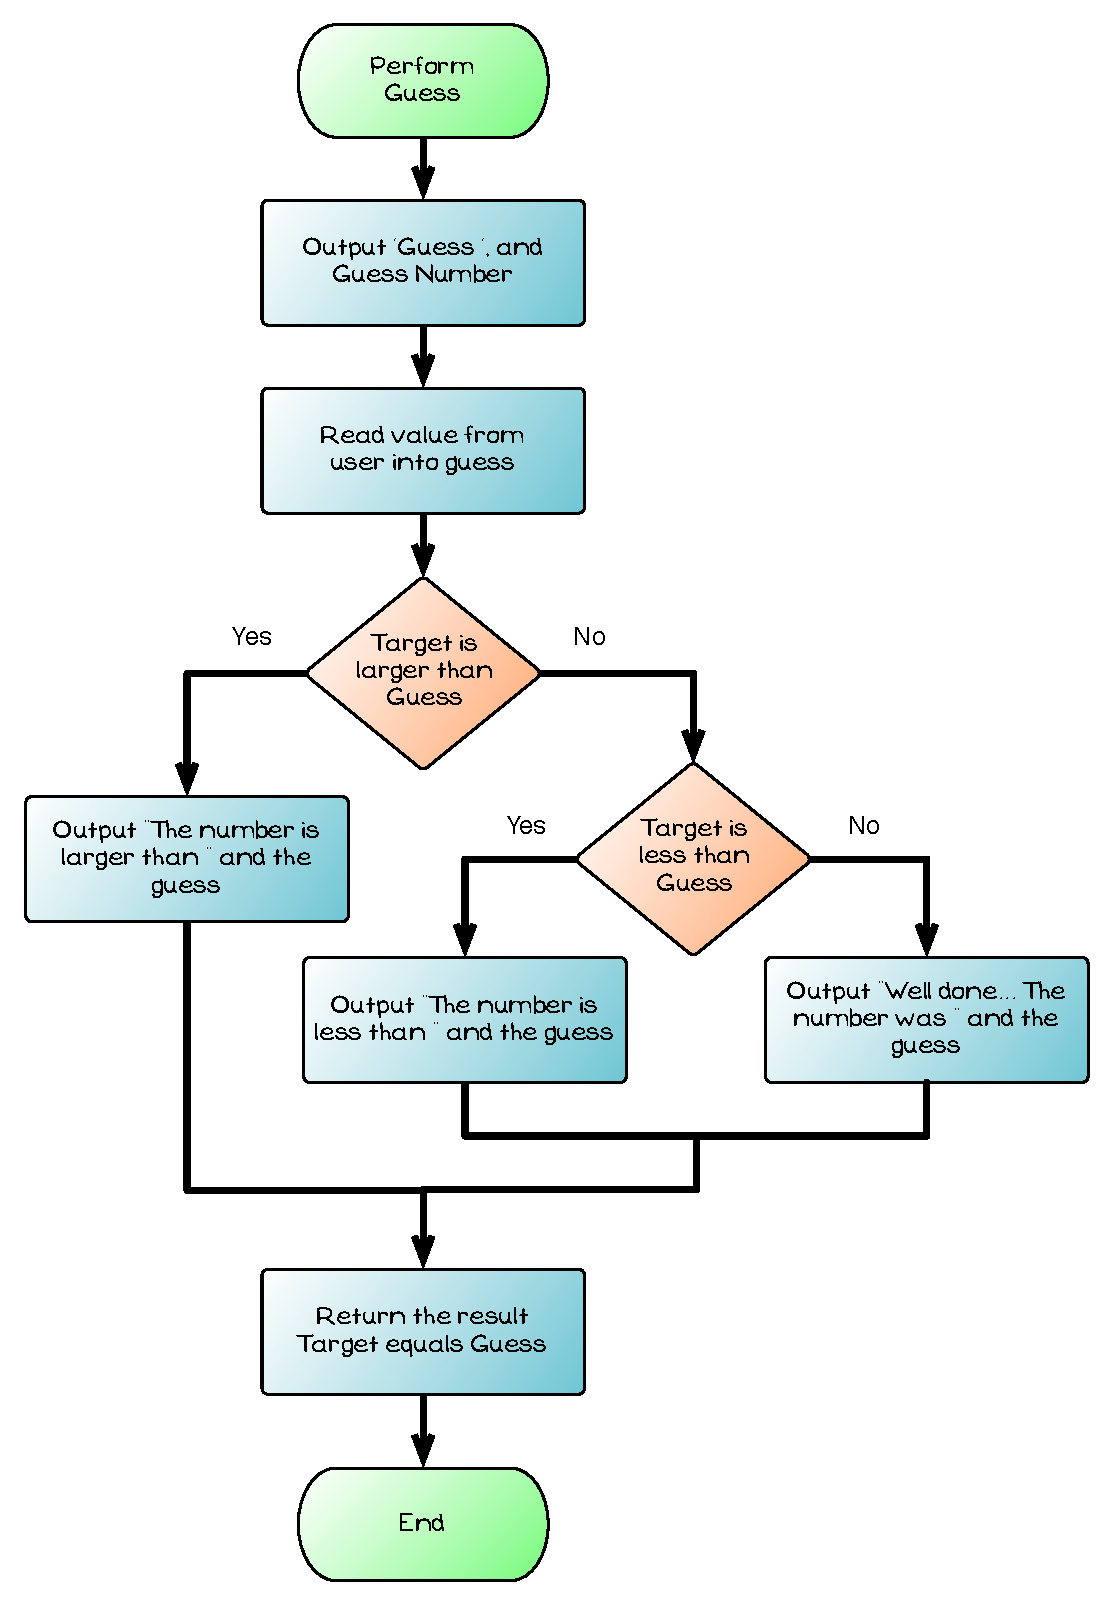
\includegraphics[width=0.5\textwidth]{./topics/control-flow/diagrams/PerformGuess5} 
   \caption{Logic for the \texttt{Perform Guess} Procedure from \fref{fig:perform-guess-5}}
   \label{fig:perform-guess-understanding}
\end{figure}

In the following illustrations \texttt{Perform Guess} will be called three times with the \texttt{target} number being \texttt{37} in each case. The following three guesses will be performed, ensuring that all paths through the flowchart are covered.
\begin{enumerate}
  \item On the first guess the user enters a guess of 50, allowing for the left most branch of this flowchart to be followed. 
  \item The second guess will be 25 to test the middle branch, taking the \emph{else} branch of the first decision and the \emph{true} branch of the second decision. 
  \item Finally the third guess will be 37, testing the right most path through the code.
\end{enumerate}


\clearpage
\subsubsection{Perform Guess is called for guess 1} % (fold)
\label{ssub:perform_guess_is_called_for_the_first_time}

In the Guess that Number program, the \texttt{Perform Guess} function is responsible for reading in the user's guess and giving them feedback. \fref{fig:perform-guess-1} shows the \texttt{Perform Guess} code being called for the first time, it is passed 1 to its \texttt{num guess} parameter and 37 to its \texttt{target} parameter.

\begin{figure}[htbp]
   \centering
   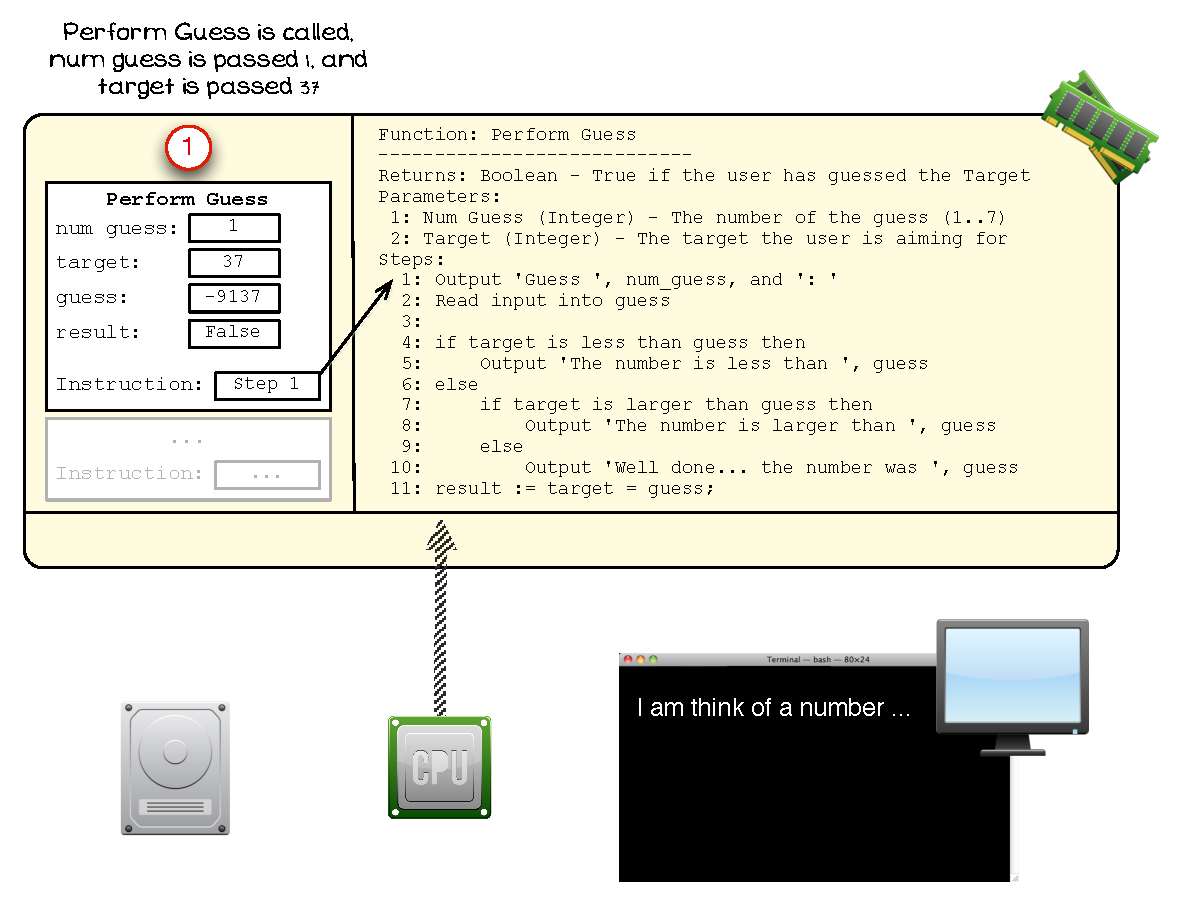
\includegraphics[width=\textwidth]{./topics/control-flow/images/PerformGuess1} 
   \caption{Perform Guess is called for the first time}
   \label{fig:perform-guess-1}
\end{figure}

\mynote{
\begin{itemize}
  \item In \fref{fig:perform-guess-1} the indicated areas show the following:
  \begin{enumerate}
    \item \texttt{Perform Guess} is called, with 1 being passed to \texttt{num guess} and 37 passed to \texttt{target}.
  \end{enumerate}
  \medskip
  \item At this point the previous code would have output `I am thinking of a number \ldots' to the Terminal.
  \item The values in \texttt{guess} and \texttt{result} have not been initialised, so they have whatever value was in that memory location previously.
\end{itemize}
}

% subsubsection perform_guess_is_called_for_the_first_time (end)
\clearpage
\subsubsection{Execution reaches the if branch for guess 1} % (fold)
\label{ssub:execution_reaches_the_if_branch}

Execution of \texttt{Perform Guess} occurs as normal, each instruction is run one after the other.

\begin{figure}[htbp]
   \centering
   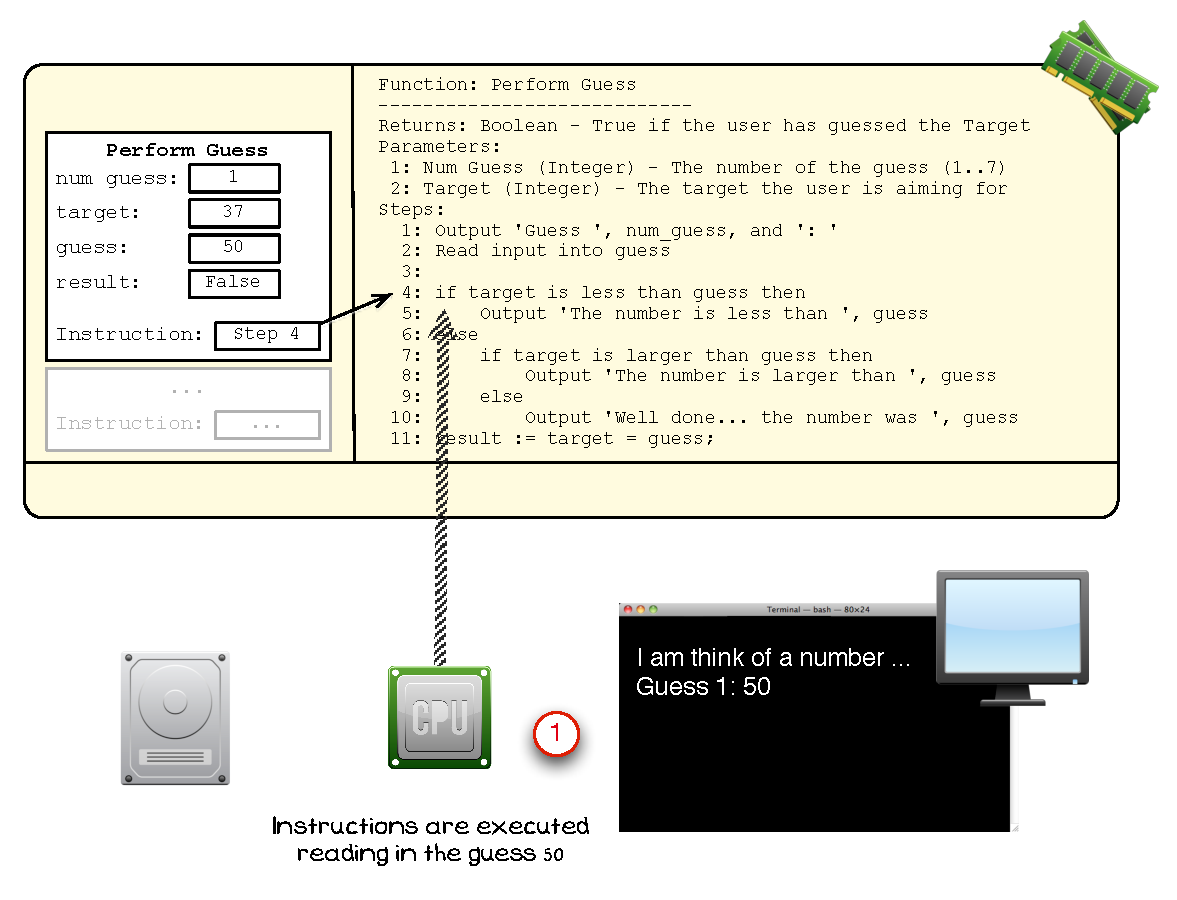
\includegraphics[width=\textwidth]{./topics/control-flow/images/PerformGuess2} 
   \caption{Program's steps are executed up to step 4}
   \label{fig:perform-guess-2}
\end{figure}

\mynote{
\begin{itemize}
  \item In \fref{fig:perform-guess-2} the indicated areas show the following:
  \begin{enumerate}
    \item Execution proceeds one instruction at a time up to the \nameref{sub:if_statement} at step 4.
  \end{enumerate}
  \medskip
  \item These steps output a prompt (step 1), and read in a response (step 2).
  \item Step 2 reads a the user's response into the \texttt{guess} variable.
  \item When the computer executes step 4 it evaluates the \nameref{sub:if_statement}'s expression and then selectively runs one of the two available paths.
\end{itemize}
}

% subsubsection execution_reaches_the_if_branch (end)
\clearpage
\subsubsection{If takes the True branch for guess 1} % (fold)
\label{ssub:if_takes_the_true_branch_for_guess_1}

With the first guess the expression in the \nameref{sub:if_statement} is \texttt{true}, \texttt{target} \textbf{is} less than \texttt{guess}. The computer jumps into the \emph{true} branch of the if statement. 

\begin{figure}[htbp]
   \centering
   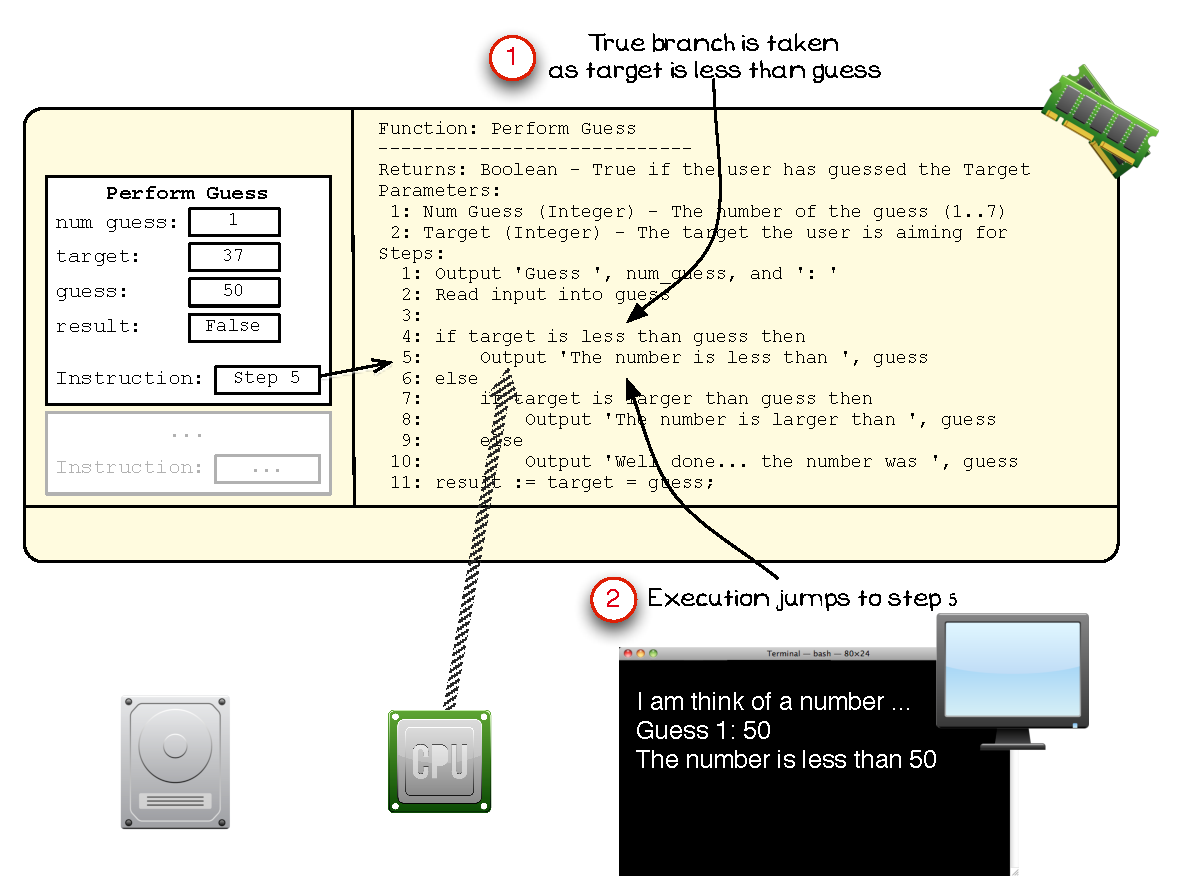
\includegraphics[width=\textwidth]{./topics/control-flow/images/PerformGuess3} 
   \caption{The \emph{true} branch is taken as \texttt{target} is less than \texttt{guess}}
   \label{fig:perform-guess-3}
\end{figure}

\mynote{
\begin{itemize}
  \item In \fref{fig:perform-guess-3} the indicated areas show the following:
  \begin{enumerate}
    \item \texttt{target} is less than \texttt{guess} so the \emph{true} branch is executed.
    \item This means the code jumps to step 5.
  \end{enumerate}
  \medskip
  \item Step 5 outputs `The number is less than 50' to the Terminal.
\end{itemize}
}

% subsubsection if_takes_the_true_branch_for_guess_1 (end)
\clearpage

\subsubsection{Control jumps to the end of \texttt{Perform Guess} for guess 1} % (fold)
\label{ssub:control_jumps_to_step_11_for_guess_1}

Once step 5 finishes, control jumps to step 11, skipping the \emph{else} branch of the if statement from step 4.

\begin{figure}[htbp]
   \centering
   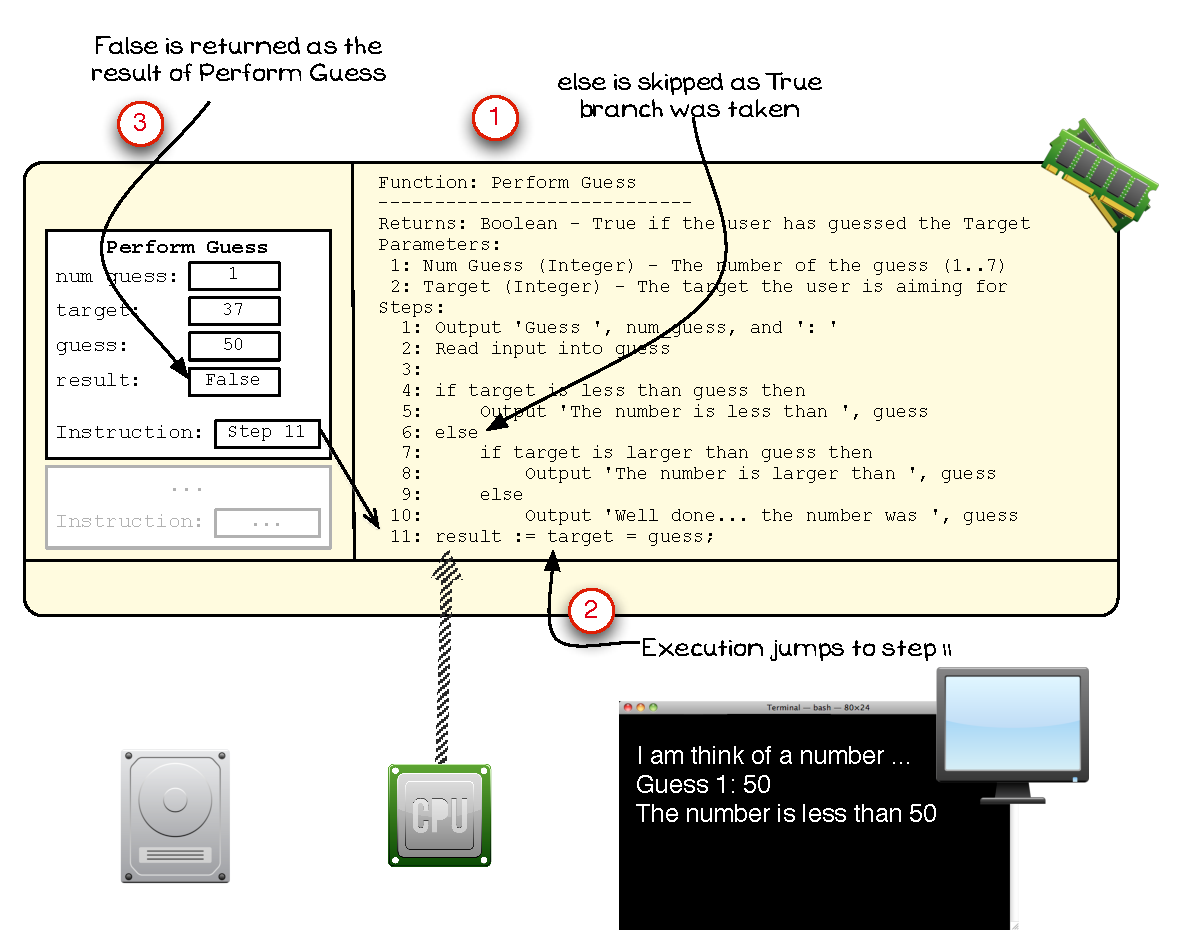
\includegraphics[width=\textwidth]{./topics/control-flow/images/PerformGuess4} 
   \caption{\texttt{Perform Guess} finishes for guess 1, returning the result \texttt{false}}
   \label{fig:perform-guess-4}
\end{figure}

\mynote{
\begin{itemize}
  \item In \fref{fig:perform-guess-4} the indicated areas show the following:
  \begin{enumerate}
    \item Steps 6 to 10 are skipped as the \emph{true} branch was taken.
    \item The next instruction is therefore step 11.
    \item This evaluates the expression \texttt{target} \textbf{equals} \texttt{guess}, which is \texttt{false}.
  \end{enumerate}
\end{itemize}
}

% subsubsection control_jumps_to_step_11_for_guess_1 (end)
\clearpage

\subsubsection{\texttt{Perform Guess} is called again for guess 2} % (fold)
\label{ssub:perform_guess_is_called_for_guess_2}

\texttt{Perform Guess} is called again, this time it is passed 2 for \texttt{guess num} and 37 for \texttt{target}. This executes the code in \texttt{Perform Guess}, one instruction at a time, eventually reaching step 4.

\begin{figure}[htbp]
   \centering
   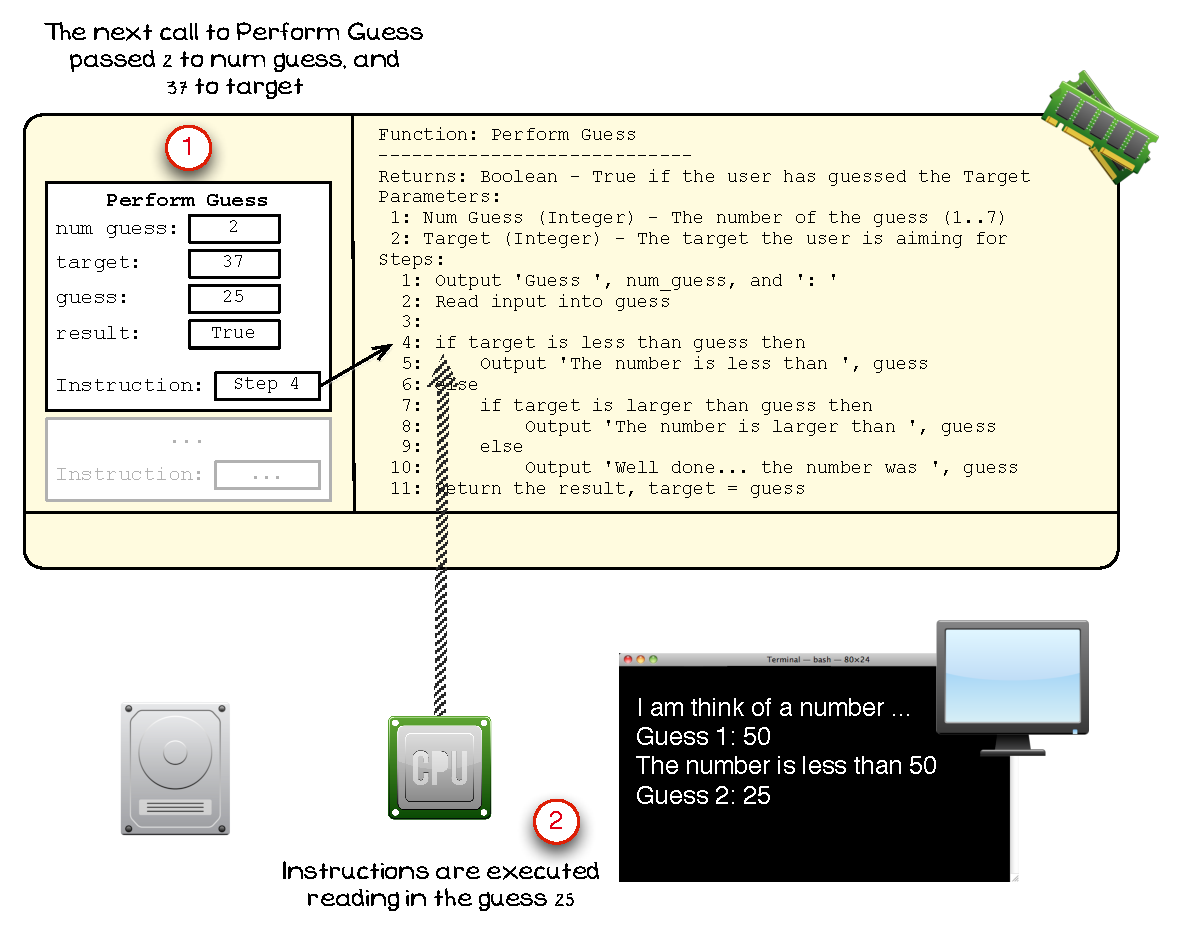
\includegraphics[width=\textwidth]{./topics/control-flow/images/PerformGuess5} 
   \caption{\texttt{Perform Guess} is run for guess 2 and advanced to step 4}
   \label{fig:perform-guess-5}
\end{figure}

\mynote{
\begin{itemize}
  \item In \fref{fig:perform-guess-5} the indicated areas show the following:
  \begin{enumerate}
    \item The call to \texttt{Perform Guess} is passed 2 for the \texttt{guess num} parameter, and 37 for the \texttt{target} parameter.
    \item The user enters 25 as their guess, this is read into the \texttt{guess} variable.
  \end{enumerate}
  \medskip
  \item The previous call ended and control returned to the caller. This is a now a new call to \texttt{Perform Guess}.
  \item Step 1 outputs a prompts for the user to enter `Guess 2: '.
  \item Step 2 reads a the user's response into the \texttt{guess} variable.
  \item When the computer executes step 4 it evaluates the \nameref{sub:if_statement}'s expression and then selectively runs one of the two available paths.
\end{itemize}
}

% subsubsection perform_guess_is_called_for_guess_2 (end)
\clearpage

\subsubsection{If takes the \emph{else} branch for guess 2} % (fold)
\label{ssub:if_takes_the_else_branch_for_guess_2}

With the second guess the expression in the \nameref{sub:if_statement} is \texttt{false}, \texttt{target} \textbf{is not} less than \texttt{guess}. The computer jumps into the \emph{else} branch of the if statement. 

\begin{figure}[htbp]
   \centering
   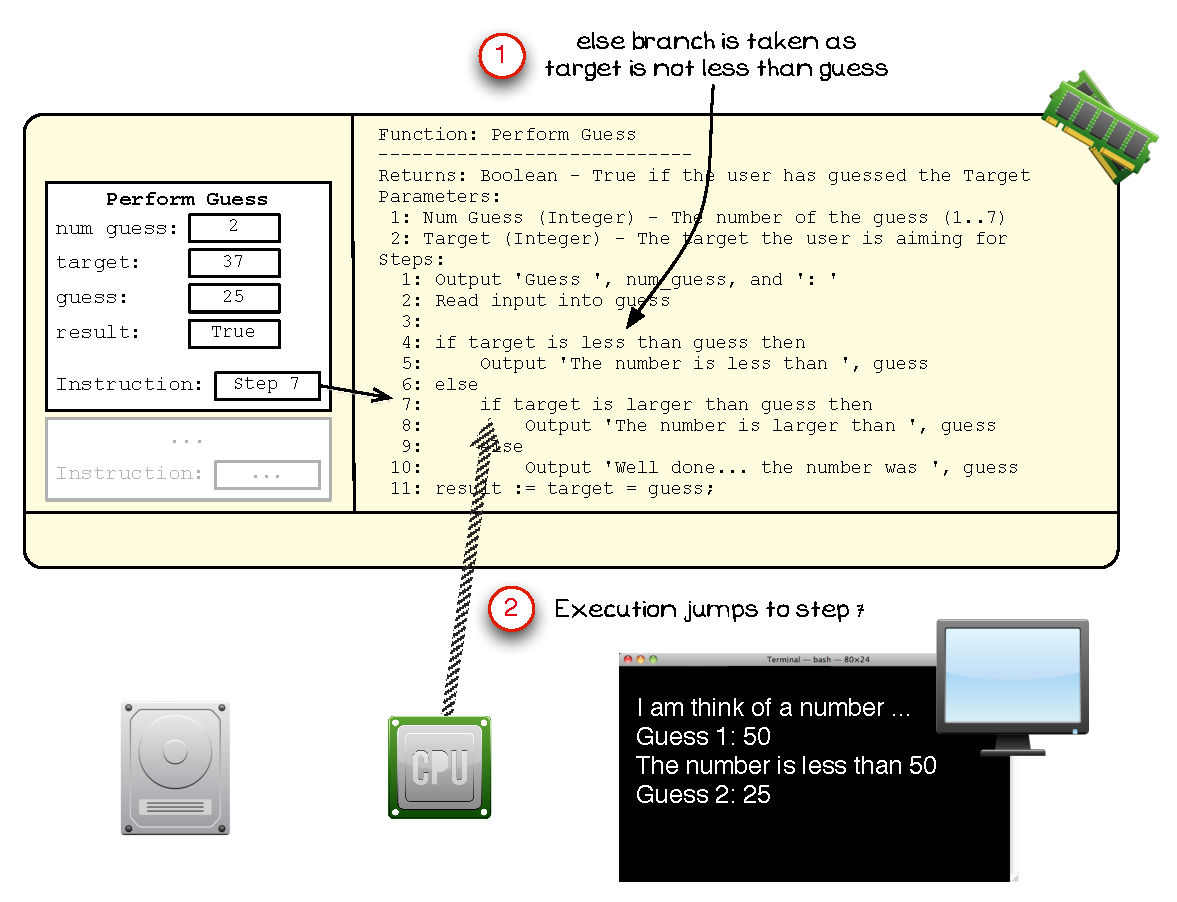
\includegraphics[width=\textwidth]{./topics/control-flow/images/PerformGuess6} 
   \caption{Control jumps to step 7 as the target is not less than the guess}
   \label{fig:perform-guess-6}
\end{figure}

\mynote{
\begin{itemize}
  \item In \fref{fig:perform-guess-6} the indicated areas show the following:
  \begin{enumerate}
    \item \texttt{target} is not less than \texttt{guess} so the \emph{else} branch is executed.
    \item This means the code jumps to step 7, skipping the \emph{true} branch.
  \end{enumerate}
  \medskip
  \item Step 7 is another \nameref{sub:if_statement}, it checks if \texttt{target} is \emph{larger} than \texttt{guess}. This expression is \texttt{true}, so it will take the \emph{true} branch next.
\end{itemize}
}

% subsubsection if_takes_the_else_branch_for_guess_2 (end)
\clearpage

\subsubsection{The inner if's \emph{true} branch is taken in guess 2} % (fold)
\label{ssub:the_inner_if_s_true_branch_is_taken_in_guess_2}

The expression in step 7 is \texttt{true}, so the if statement directs the computer into the \emph{true} branch at step 8.

\begin{figure}[htbp]
   \centering
   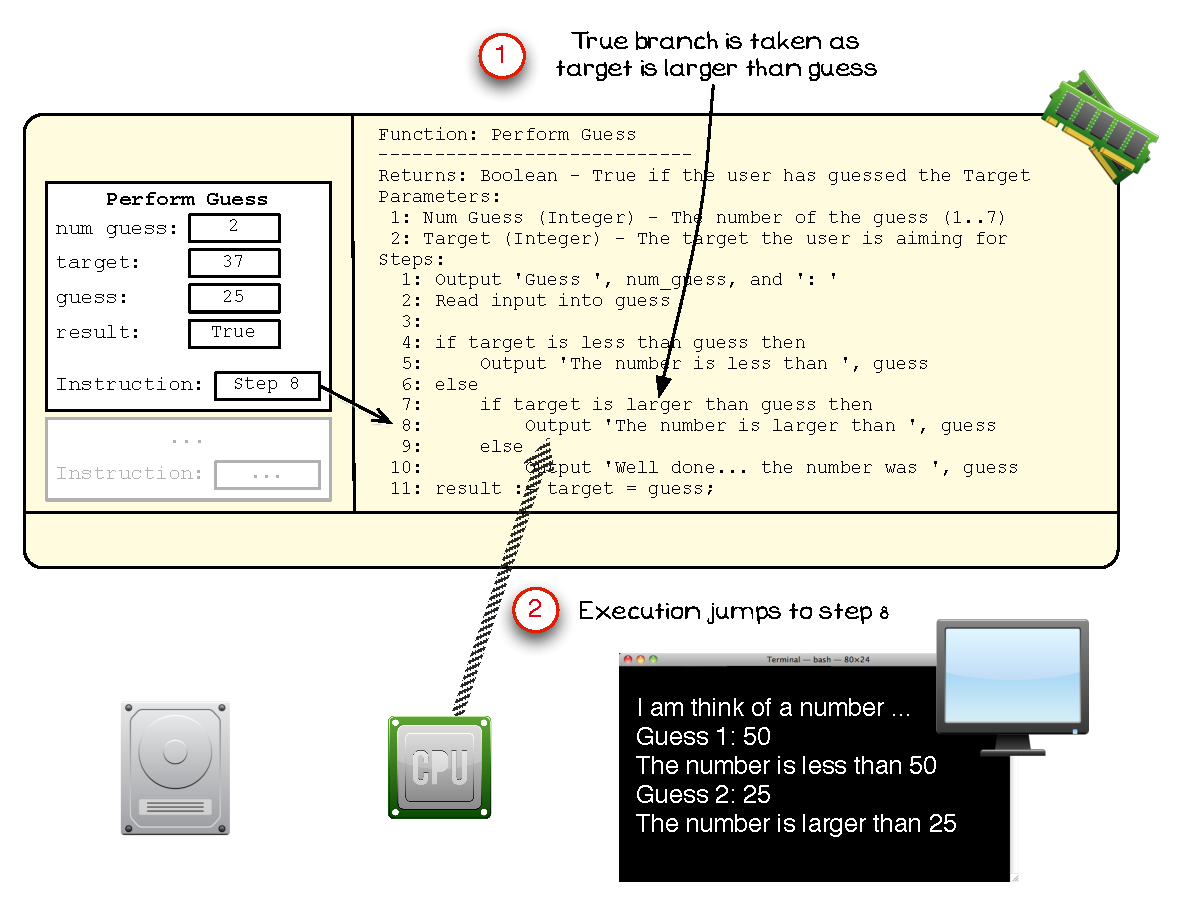
\includegraphics[width=\textwidth]{./topics/control-flow/images/PerformGuess7} 
   \caption{Control continues into the \emph{true} branch of the inner if statement}
   \label{fig:perform-guess-7}
\end{figure}

\mynote{
\begin{itemize}
  \item In \fref{fig:perform-guess-7} the indicated areas show the following:
  \begin{enumerate}
    \item \texttt{target} is larger than \texttt{guess} so the \emph{true} branch is taken.
    \item This means the code jumps to step 8.
  \end{enumerate}
  \medskip
  \item Step 8 outputs the message `The number if larger than 25' to the Terminal.
\end{itemize}
}

% subsubsection the_inner_if_s_true_branch_is_taken_in_guess_2 (end)
\clearpage

\subsubsection{Control jumps to the end of \texttt{Perform Guess} for guess 2} % (fold)
\label{ssub:control_jumps_to_step_11_for_guess_2}

Once step 8 finishes, control jumps to step 11, skipping the \emph{else} branch of the if statement from step 7 and also ending the if statement started at step 4.

\begin{figure}[htbp]
   \centering
   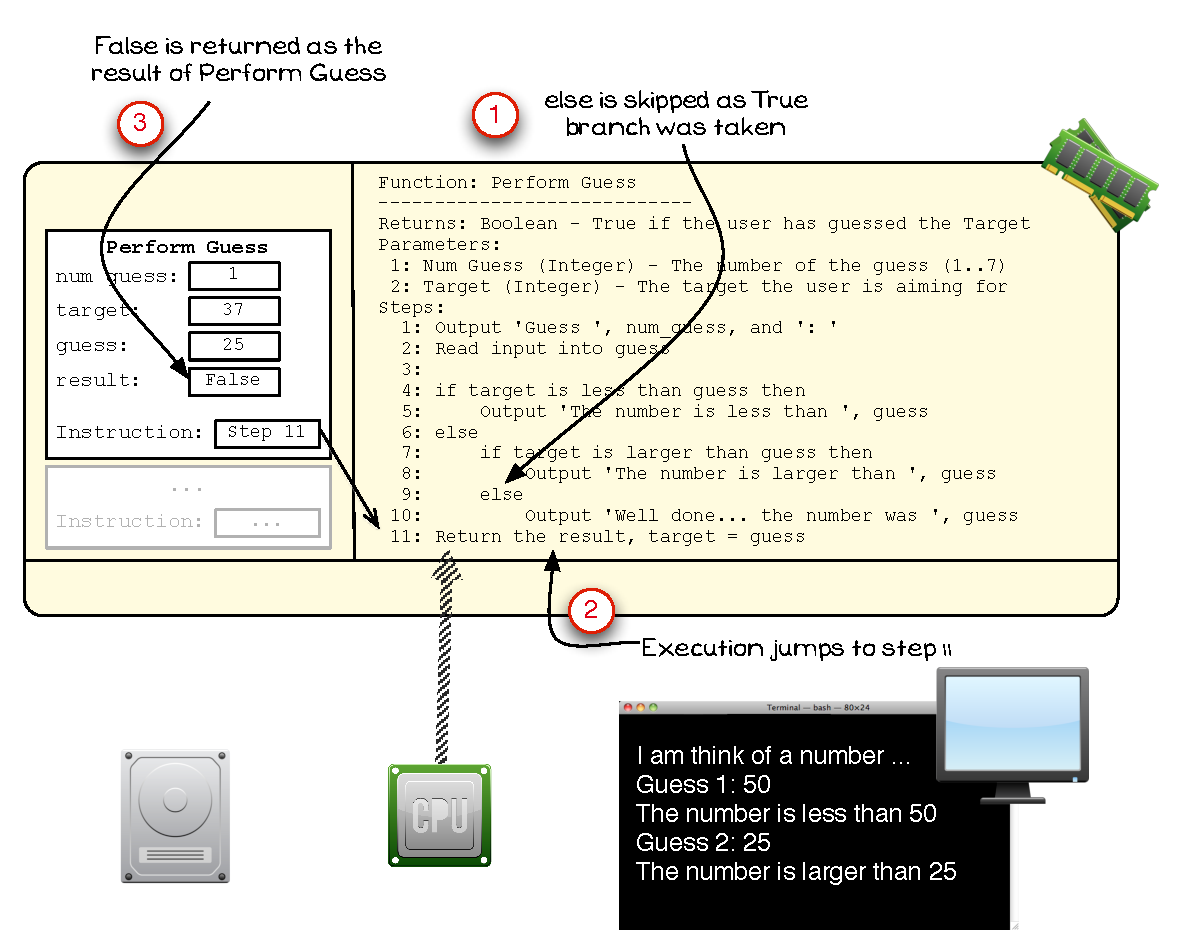
\includegraphics[width=\textwidth]{./topics/control-flow/images/PerformGuess8} 
   \caption{Guess 2 ends with \texttt{Perform Guess} returning \texttt{False}}
   \label{fig:perform-guess-8}
\end{figure}

\mynote{
\begin{itemize}
  \item In \fref{fig:perform-guess-8} the indicated areas show the following:
  \begin{enumerate}
    \item The else branch starting at step 9 is skipped as the \emph{true} branch was taken.
    \item The next instruction is therefore step 11, ending the if statements starts at steps 7 and 4.
    \item \texttt{Perform Guess} returns the result \texttt{false} as the expression \texttt{target} equals \texttt{guess} is \texttt{false}.
  \end{enumerate}
\end{itemize}
}

% subsubsection control_jumps_to_step_11_for_guess_2 (end)
\clearpage

\subsubsection{Perform Guess is called again for guess 3} % (fold)
\label{ssub:perform_guess_is_called_again_for_guess_3}

\texttt{Perform Guess} is called again, this time it is passed 3 for \texttt{guess num} and 37 for \texttt{target}. This executes the code in \texttt{Perform Guess}, one instruction at a time, eventually reaching step 4.

\begin{figure}[htbp]
   \centering
   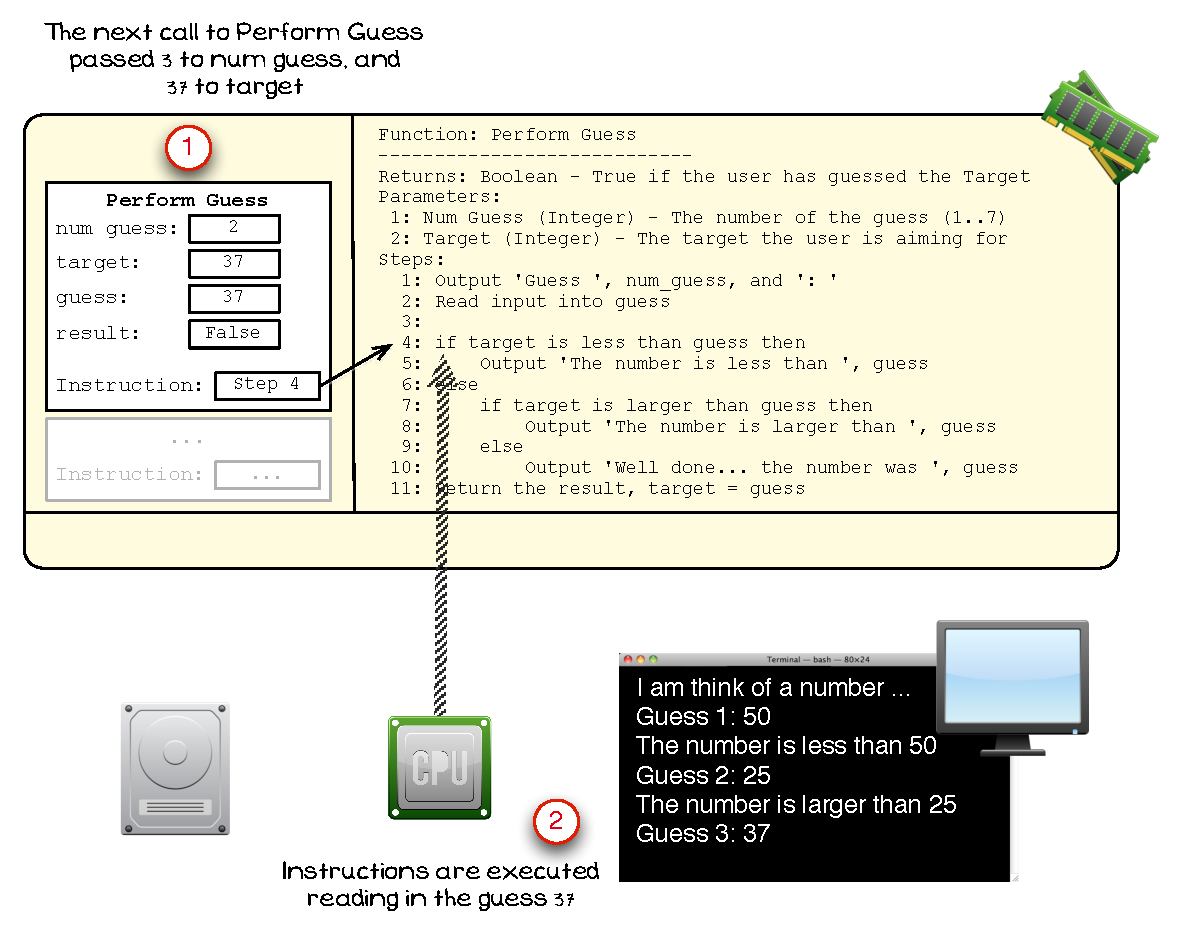
\includegraphics[width=\textwidth]{./topics/control-flow/images/PerformGuess9} 
   \caption{\texttt{Perform Guess} is run for guess 3 and advanced to step 4}
   \label{fig:perform-guess-9}
\end{figure}

\mynote{
\begin{itemize}
  \item In \fref{fig:perform-guess-9} the indicated areas show the following:
  \begin{enumerate}
    \item The call to \texttt{Perform Guess} is passed 3 for the \texttt{guess num} parameter, and 37 for the \texttt{target} parameter.
    \item The user enters 37 as their guess, this is read into the \texttt{guess} variable.
  \end{enumerate}
  \medskip
  \item The previous call ended and control returned to the caller. This is a now a new call to \texttt{Perform Guess}.
  \item Step 1 outputs a prompts for the user to enter `Guess 3: '.
  \item Step 2 reads a the user's response into the \texttt{guess} variable.
  \item When the computer executes step 4 it evaluates the \nameref{sub:if_statement}'s expression and then selectively runs one of the two available paths. In this case the expression is \texttt{false} as \texttt{target} is not less than \texttt{guess}.
\end{itemize}
}

% subsubsection perform_guess_is_called_again_for_guess_3 (end)
\clearpage

\subsubsection{If takes the \emph{else} branch for guess 3} % (fold)
\label{ssub:if_takes_the_else_branch_for_guess_3}

The \texttt{target} is \textbf{not} less than the user's guess, so the \emph{else} branch of the if statement at step 4 is taken, with the computer jumping to step 7.

\begin{figure}[htbp]
   \centering
   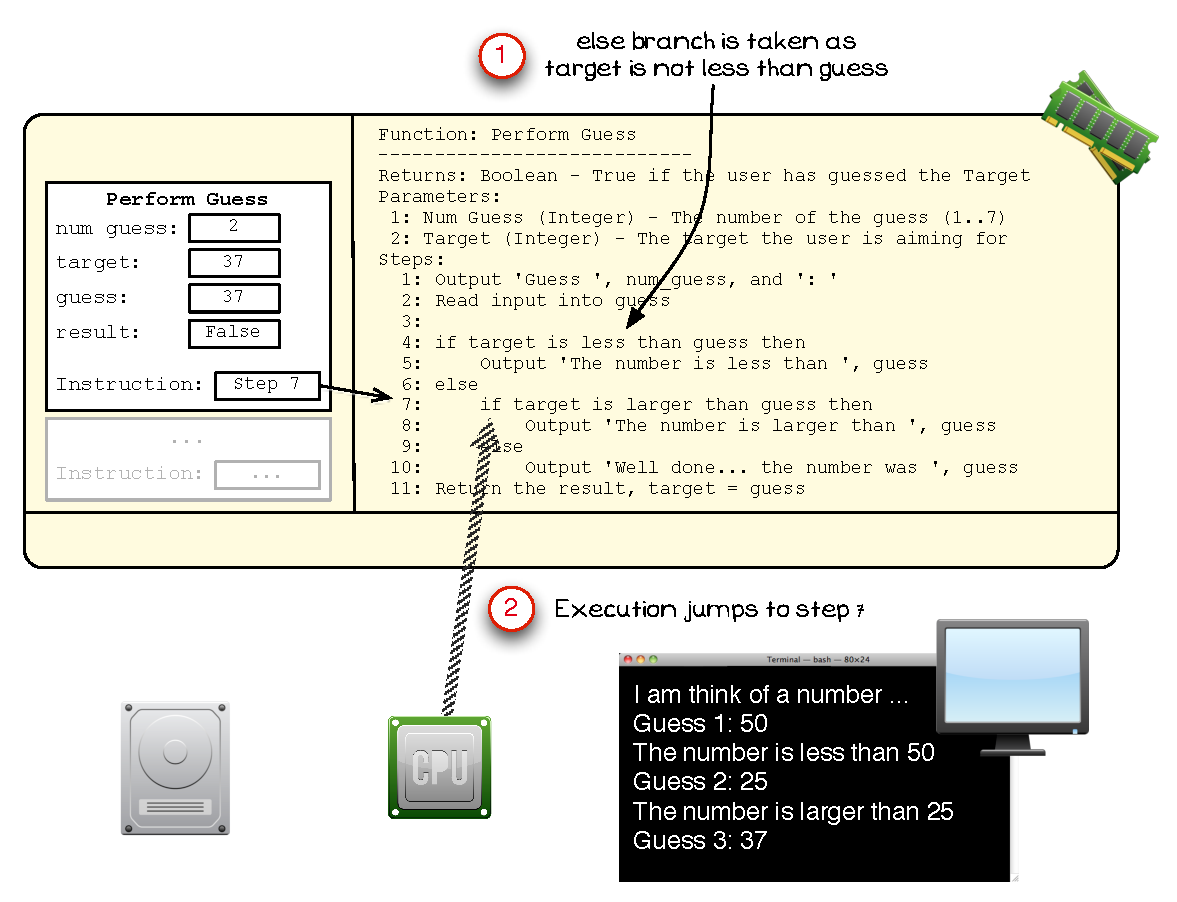
\includegraphics[width=\textwidth]{./topics/control-flow/images/PerformGuess10} 
   \caption{The \emph{else} branch is taken as \texttt{target} is not less than \texttt{guess} for guess 3}
   \label{fig:perform-guess-10}
\end{figure}

\mynote{
\begin{itemize}
  \item In \fref{fig:perform-guess-10} the indicated areas show the following:
  \begin{enumerate}
    \item \texttt{target} is not less than \texttt{guess} so the \emph{else} branch is executed.
    \item This means the code jumps to step 7, skipping the \emph{true} branch.
  \end{enumerate}
  \medskip
  \item Step 7 is another \nameref{sub:if_statement}, it checks if \texttt{target} is \emph{larger} than \texttt{guess}. This expression is also \texttt{false}, \texttt{target} is \emph{not} larger than \texttt{guess}.
\end{itemize}
}

% subsubsection if_takes_the_else_branch_for_guess_3 (end)
\clearpage

\subsubsection{The inner if's \emph{else} branch is taken in guess 3} % (fold)
\label{ssub:the_inner_if_s_else_branch_is_taken_in_guess_3}

The \texttt{target} is \textbf{not} larger than the user's guess, so the \emph{else} branch of the if statement at step 7 is taken, with the computer jumping to step 10.

\begin{figure}[htbp]
   \centering
   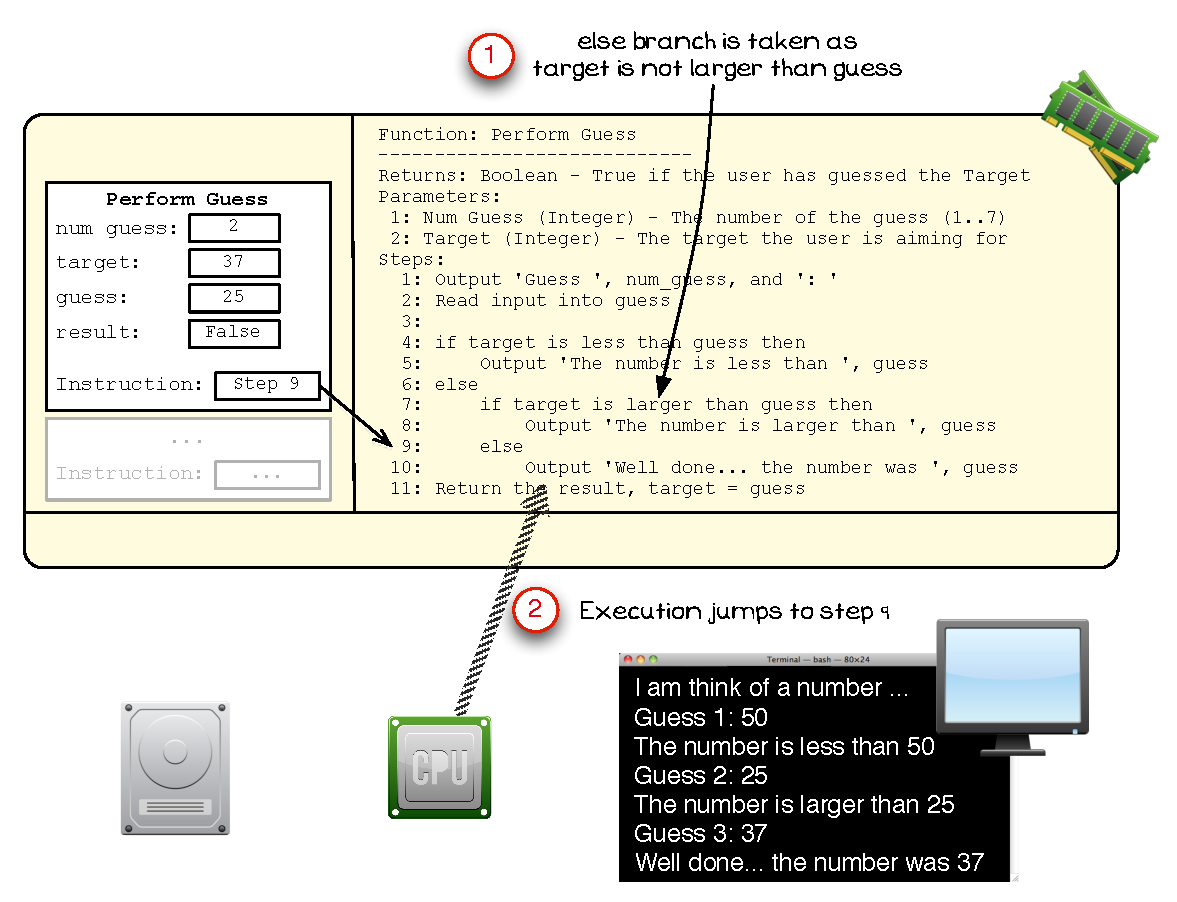
\includegraphics[width=\textwidth]{./topics/control-flow/images/PerformGuess11} 
   \caption{The \texttt{target} is not larger than \texttt{guess}, so the \emph{else} branch of the if statement at step 7 is taken.}
   \label{fig:perform-guess-11}
\end{figure}

\mynote{
\begin{itemize}
  \item In \fref{fig:perform-guess-11} the indicated areas show the following:
  \begin{enumerate}
    \item \texttt{target} is not larger than \texttt{guess} so the \emph{else} branch is executed.
    \item This means the code jumps to step 10, skipping the \emph{true} branch.
  \end{enumerate}
  \medskip
  \item Step 10 outputs `Well done\ldots the number was 37' to the Terminal.
\end{itemize}
}

% subsubsection the_inner_if_s_else_branch_is_taken_in_guess_3 (end)
\clearpage

\subsubsection{Control jumps to the end of \texttt{Perform Guess} for guess 3} % (fold)
\label{ssub:control_jumps_to_step_11_for_guess_3}

Once step 10 finishes, control jumps to step 11, ending the if statements from step 7 and step~ 4.

\begin{figure}[htbp]
   \centering
   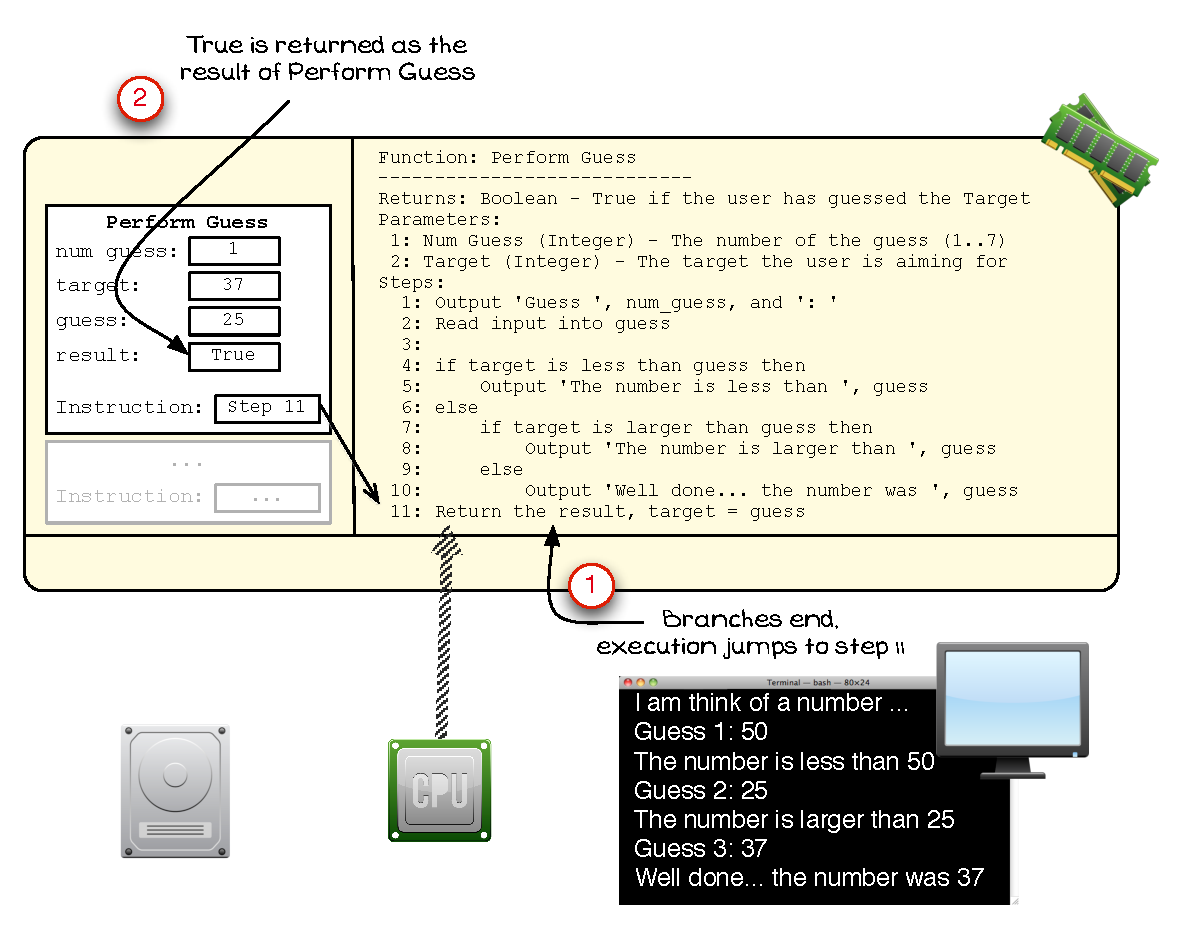
\includegraphics[width=\textwidth]{./topics/control-flow/images/PerformGuess12} 
   \caption{Program's entry point is loaded onto the Stack}
   \label{fig:perform-guess-12}
\end{figure}

\mynote{
\begin{itemize}
  \item In \fref{fig:perform-guess-12} the indicated areas show the following:
  \begin{enumerate}
    \item The if statements at steps 7 and 4 end, with control jumping to step 11.
    \item The result returned will be \texttt{true}, \texttt{target} does equal \texttt{guess}.
  \end{enumerate}
  
\end{itemize}
}

% subsubsection control_jumps_to_step_11_for_guess_3 (end)
% subsection understanding_branching_in_perform_guess (end)

\clearpage
\subsection{Understanding Looping in Play Game} % (fold)
\label{sub:understanding_looping_in_play_game}

\fref{fig:play-game-understanding} shows the flowchart for the \texttt{Play Game} procedure that was developed in \sref{sub:designing_control_flow_for_play_game} on \nameref{sub:designing_control_flow_for_play_game}. The following sections outline how these actions are executed within the computer.

\begin{figure}[htbp]
   \centering
   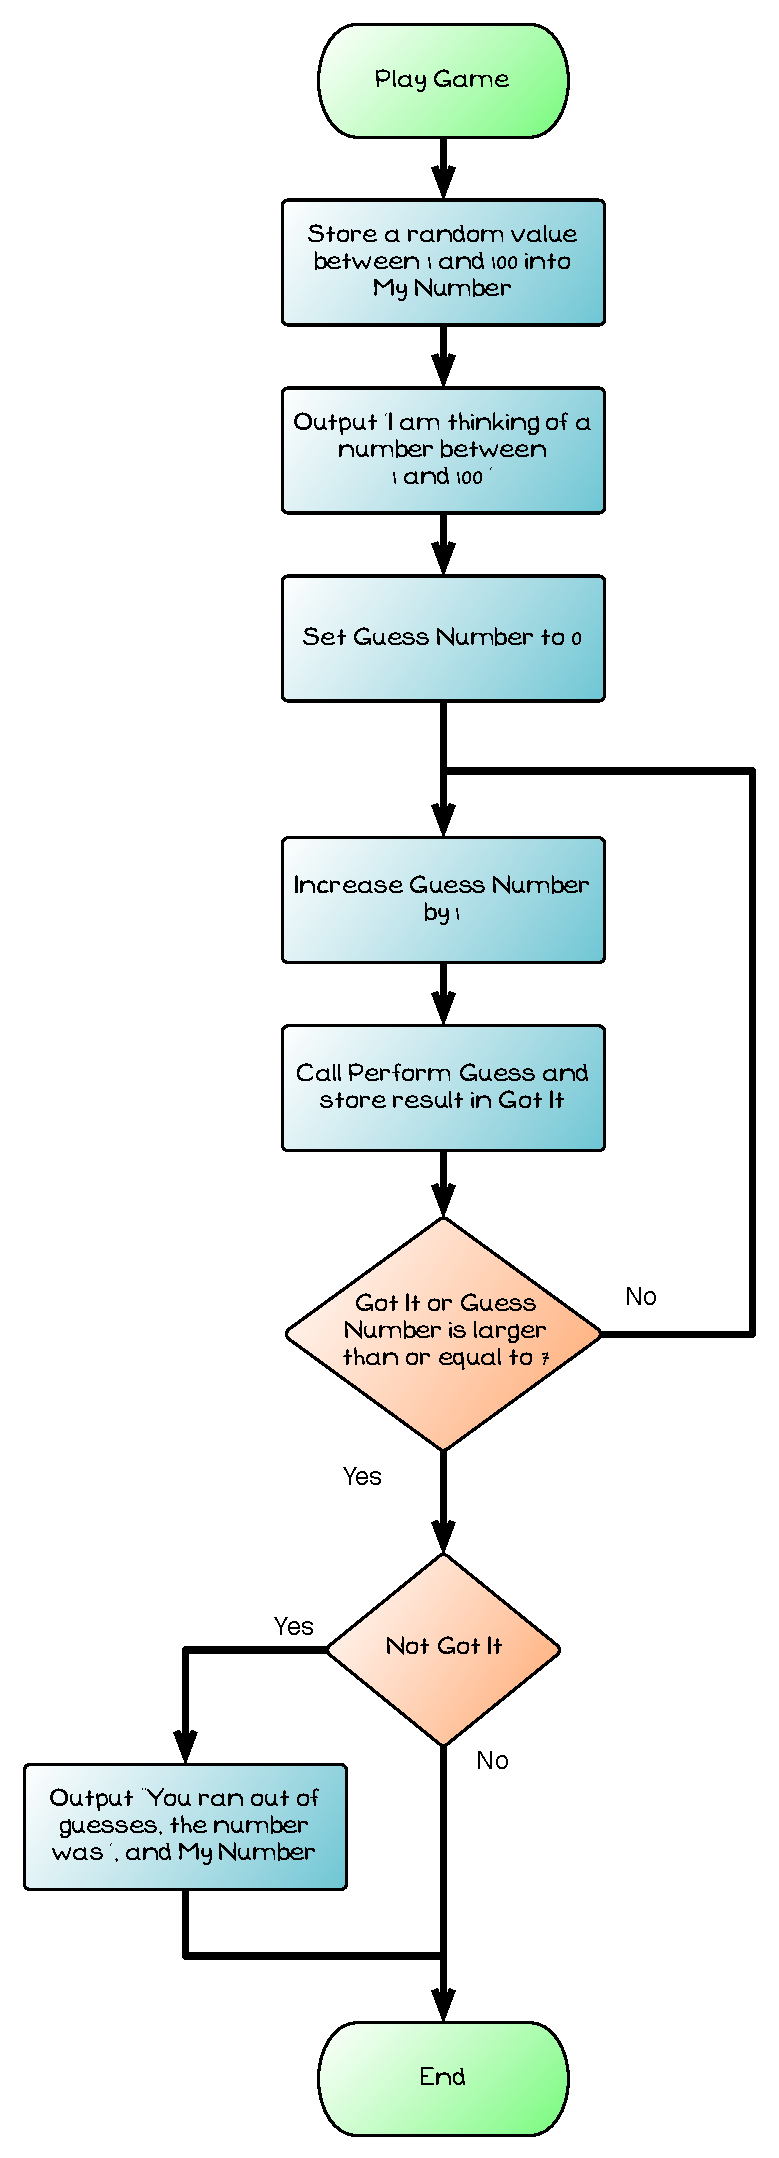
\includegraphics[width=0.38\textwidth]{./topics/control-flow/diagrams/PlayGame} 
   \caption{Logic for the \texttt{Play Game} Procedure from \fref{fig:play-game}}
   \label{fig:play-game-understanding}
\end{figure}

In the following illustrations \texttt{Play Game} will be called once, and will perform three guesses. These three guesses match the calls illustrated in \sref{sub:understanding_branching_in_perform_guess} \nameref{sub:understanding_branching_in_perform_guess}. In each case the details of the call into \texttt{Perform Guess} will not be recovered, but you can refer back to the previous section if needed. 

The illustrations will show how the loop in the flowchart is handled by the computer. As this includes a \texttt{do...while}/\texttt{repeat...until} loop, the explanations will present both boolean expressions. Please ensure that you check the logic based on the implementation you will use.

\clearpage
\subsubsection{\texttt{Play Game} is called} % (fold)
\label{ssub:play game_is_called}

At some point the \texttt{Play Game} procedure is called. This will be responsible for coordinating the actions needed to play one game of Guess that Number. It will call \texttt{Perform Guess} to do the work needed to perform each individual guess.

\begin{figure}[htbp]
   \centering
   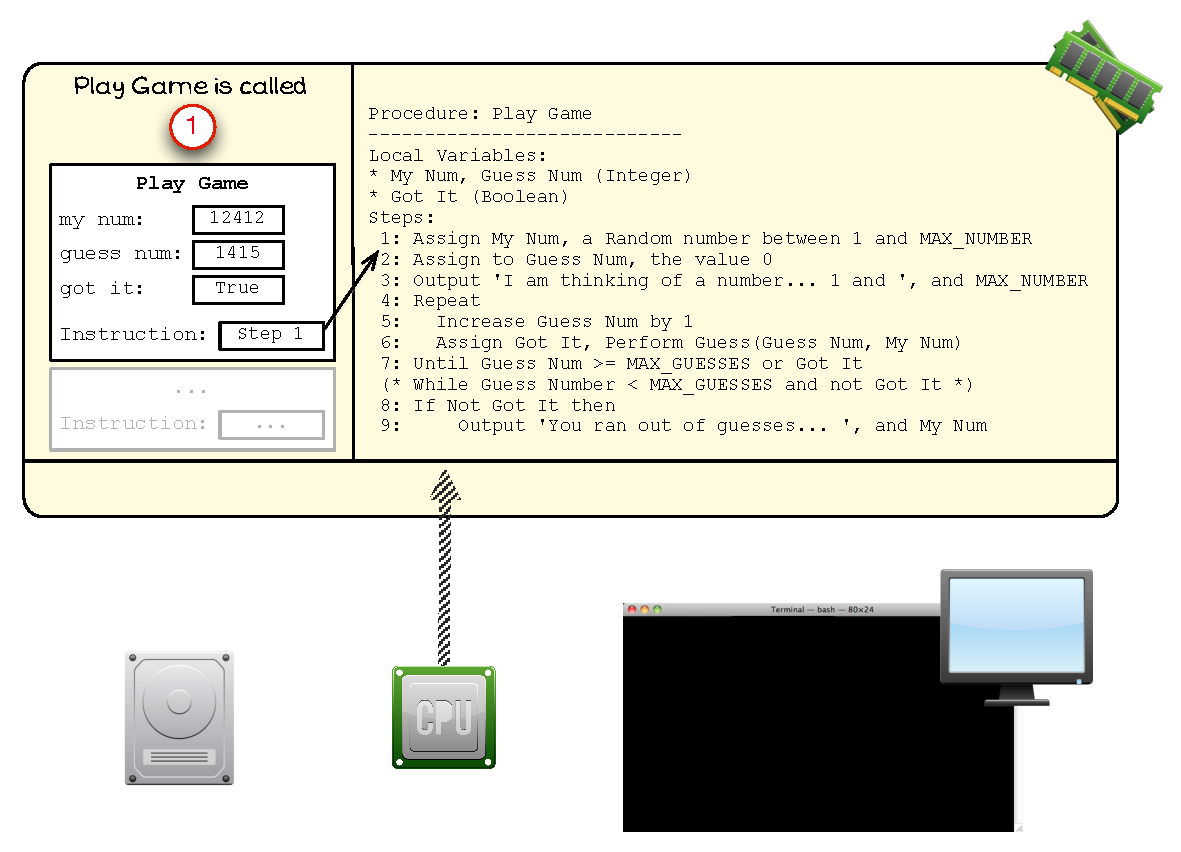
\includegraphics[width=\textwidth]{./topics/control-flow/images/PlayGame1} 
   \caption{\texttt{Play Game} is called, it is allocated space on the Stack for its local variables}
   \label{fig:play-game-1}
\end{figure}

\mynote{
\begin{itemize}
  \item In \fref{fig:play-game-1} the indicated areas show the following:
  \begin{enumerate}
    \item \texttt{Play Game} is allocated spaces on the stack for its local variables.
  \end{enumerate}
  \medskip
  \item Local variables are not initialised, so their values are whatever happened to be at that location in memory before.
  \item Step 1 generates a random number and stores this in \texttt{my num}.
  \item Step 2 initialises the value of \texttt{guess num} with the value 0.
  \item Step 3 will output a message indicating the start of the game.
\end{itemize}
}

% subsubsection play game_is_called (end)
\clearpage

\subsubsection{The loop is entered} % (fold)
\label{ssub:control_runs_to_step_4}

Steps 1 to 3 execute and initialise the \texttt{my num} and \texttt{guess num} local variables. 

\begin{figure}[htbp]
   \centering
   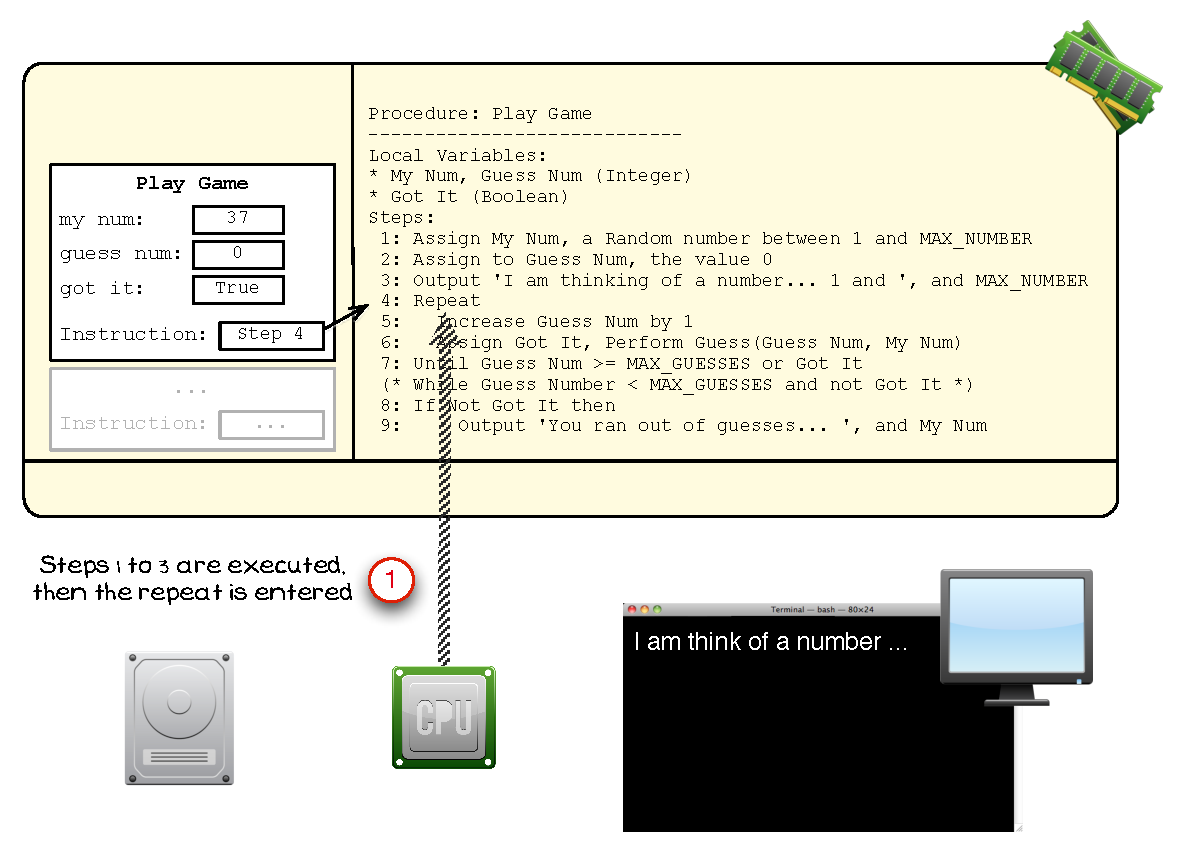
\includegraphics[width=\textwidth]{./topics/control-flow/images/PlayGame2} 
   \caption{}
   \label{fig:play-game-2}
\end{figure}

\mynote{
\begin{itemize}
  \item In \fref{fig:play-game-2} the indicated areas show the following:
  \begin{enumerate}
    \item Steps 1 to 3 are executed, and then control enters the repeated block.
  \end{enumerate}
  \medskip
  \item The repeated instructions will continue as normal.
  \item If this were a \nameref{sub:pre_test_loop}, the condition would be checked \emph{before} the loop body was executed. Other than that the two kinds of loops are the same.
\end{itemize}
}

\csection{Remember that in C the \nameref{sub:post_test_loop} is the \nameref{sub:c_do_while_loop}. This is similar to \texttt{repeat \ldots until}, differing only in the way the boolean condition is expressed.}

\passection{Remember that in Pascal the \nameref{sub:post_test_loop} is \texttt{repeat...until}. This is similar to \texttt{do \ldots while}, differing only in the way the boolean condition is expressed.}


% subsubsection control_runs_to_step_4 (end)

\clearpage
\subsubsection{\texttt{Perform Guess} is called, and returns false for guess 1} % (fold)
\label{ssub:perform guess_returns_false_for_guess_1}

\begin{figure}[htbp]
   \centering
   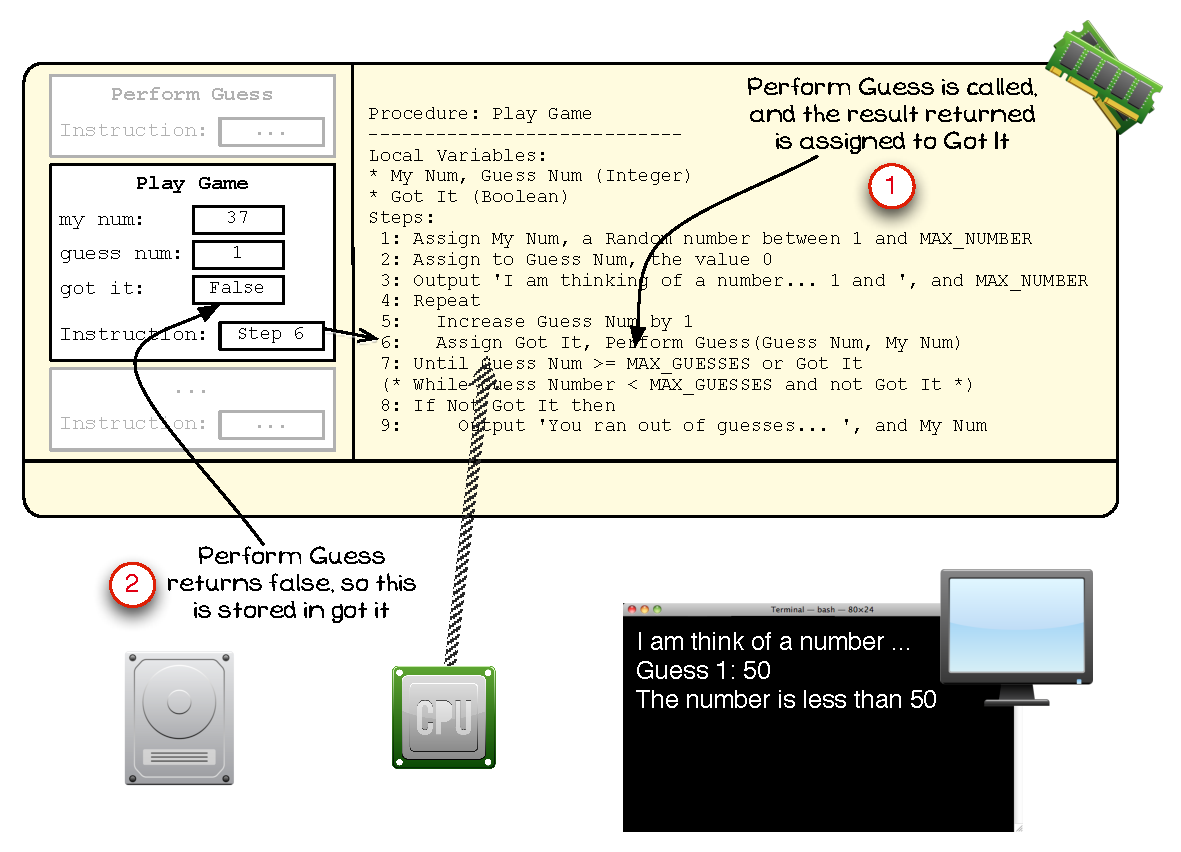
\includegraphics[width=\textwidth]{./topics/control-flow/images/PlayGame3} 
   \caption{}
   \label{fig:play-game-3}
\end{figure}

\mynote{
\begin{itemize}
  \item In \fref{fig:play-game-3} the indicated areas show the following:
  \begin{enumerate}
    \item This calls \texttt{Perform Guess} passing 1 to its \texttt{guess num} parameter, and 37 to its \texttt{target} parameter.
    \item \texttt{Perform Guess} returns \texttt{false}, indicating that the user did not guess the number.
  \end{enumerate}
  \medskip
  \item The following sections outline what occurred in \texttt{Perform Guess}:
  \begin{itemize}
    \item \nameref{ssub:perform_guess_is_called_for_the_first_time}
    \item \nameref{ssub:execution_reaches_the_if_branch}
    \item \nameref{ssub:if_takes_the_true_branch_for_guess_1}
    \item \nameref{ssub:control_jumps_to_step_11_for_guess_1}
  \end{itemize}
\end{itemize}
}

% subsubsection perform guess_returns_false_for_guess_1 (end)

\clearpage
\subsubsection{Loop condition is checked at the end of guess 1, with the loop being repeated} % (fold)
\label{ssub:loop_condition_is_checked_at_the_end_of_guess_1}

At the end of the loop the condition is checked, in this case the loop will run again.

\begin{figure}[htbp]
   \centering
   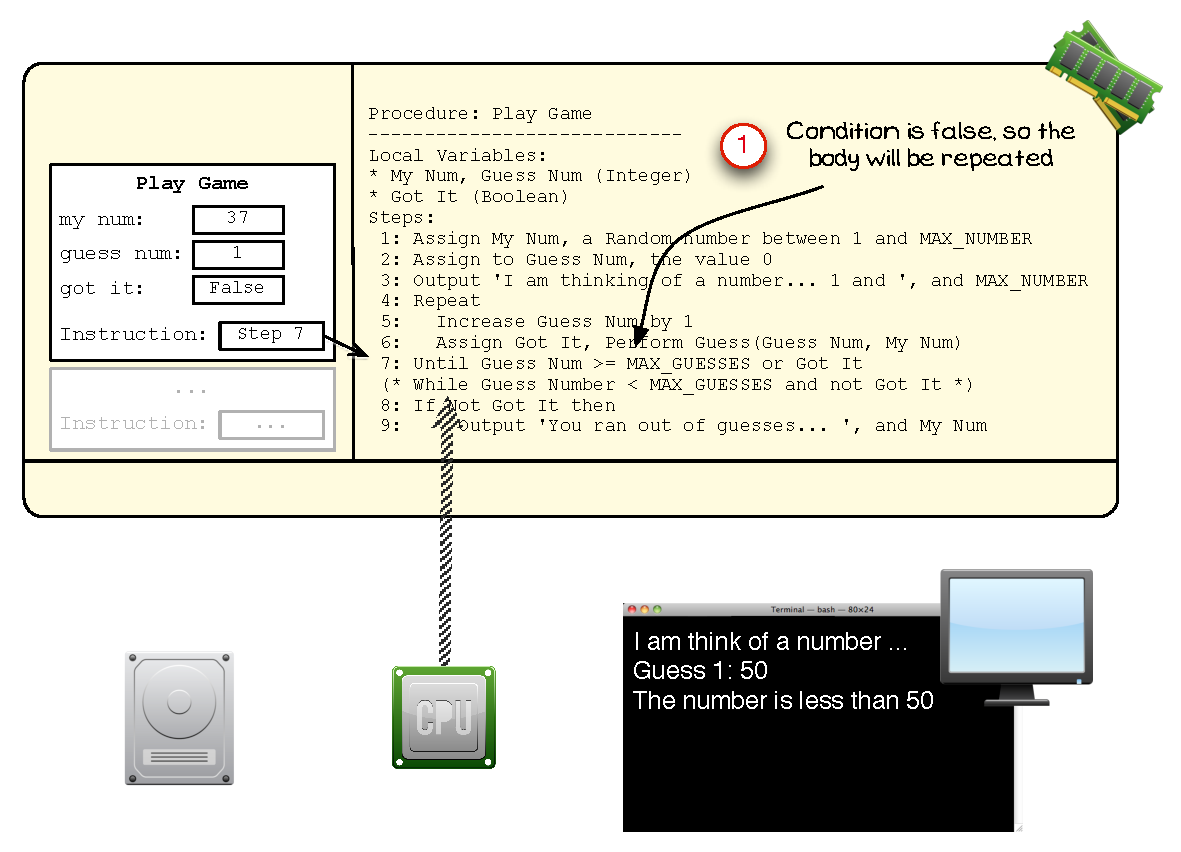
\includegraphics[width=\textwidth]{./topics/control-flow/images/PlayGame4} 
   \caption{Condition indicates that the loop's body should be executed again}
   \label{fig:play-game-4}
\end{figure}

\mynote{
\begin{itemize}
  \item In \fref{fig:play-game-4} the indicated areas show the following:
  \begin{enumerate}
    \item The condition is checked, and the expression is \texttt{false}. 
  \end{enumerate}
  \medskip
  \item With \texttt{\textbf{repeat...until}} you can evaluate the expression by:
  \begin{enumerate}
    \item \csnipet{Guess Num >= MAX\_GUESSES} is \csnipet{1 >= 7}, this is \textbf{false}
    \item \texttt{Got it}, this is a variable, its value is \textbf{false}
    \item Or the above together, \passnipet{false or false}, this is \textbf{false}, repeating the loop.
  \end{enumerate}
  \item With \texttt{\textbf{do...while}} you can evaluate the expression by:
  \begin{enumerate}
    \item \csnipet{Guess Num < MAX\_GUESSES} is \csnipet{1 < 7}, this is \textbf{true}
    \item \texttt{Got it}, this is a variable, its value is \emph{false}, so \texttt{!Got it}, is \texttt{not false}, is \textbf{true}
    \item And together these results, \passnipet{true and true} is \textbf{true}, repeating the loop.
  \end{enumerate}
\end{itemize}
}

\csection{For C you will need to code this as a \nameref{sub:c_do_while_loop}. The code for this will be \csnipet{do...while(guess\_num < MAX\_GUESSES && !got\_it);}}

\passection{For Pascal you will need to code this as a Pascal Repeat Until Loop. The code for this will be \passnipet{repeat...until (guess\_num >= MAX\_GUESSES) or (got\_it);}}

% subsubsection loop_condition_is_checked_at_the_end_of_guess_1 (end) 

\clearpage
\subsubsection{Control returns to the top of the loop to perform guess 2} % (fold)
\label{ssub:control_returns_to_the_top_of_the_loop_to_perform_guess_2}

The loop repeats to perform guess 2.

\begin{figure}[htbp]
   \centering
   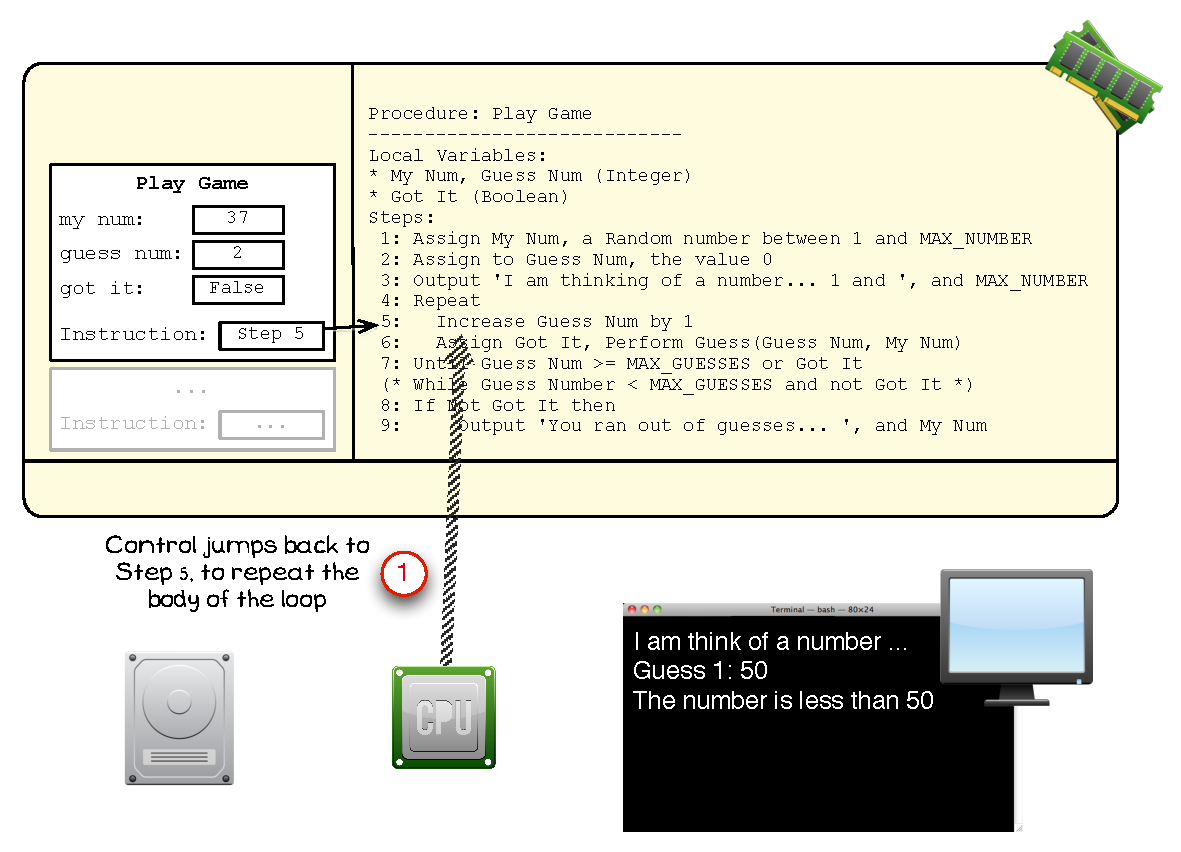
\includegraphics[width=\textwidth]{./topics/control-flow/images/PlayGame5} 
   \caption{Control returns to step 5 to repeat the body of the loop}
   \label{fig:play-game-5}
\end{figure}

\mynote{
\begin{itemize}
  \item In \fref{fig:play-game-5} the indicated areas show the following:
  \begin{enumerate}
    \item The loop's body starts at step 5, so control jumps back to this point to repeat the instructions in the loop.
  \end{enumerate}
  \medskip
  \item Step 5 increases the value of the \texttt{guess num} local variable.
\end{itemize}
}

% subsubsection control_returns_to_the_top_of_the_loop_to_perform_guess_2 (end)

\clearpage
\subsubsection{\texttt{Perform Guess} is called again, and returns false for guess 2} % (fold)
\label{ssub:perform_guess_is_called_to_perform_guess_2}

In the body of the loop, step 5 increases the value in \texttt{guess num} to 2 then control continues to step 6. This step calls \texttt{Perform Guess}, to allow the user to perform the second guess. This time around it is passed 2 for the \texttt{guess num}, and 37 for the \texttt{target}. When \texttt{Perform Guess} ends the result is false again, which is stored in \texttt{got it}.

\begin{figure}[htbp]
   \centering
   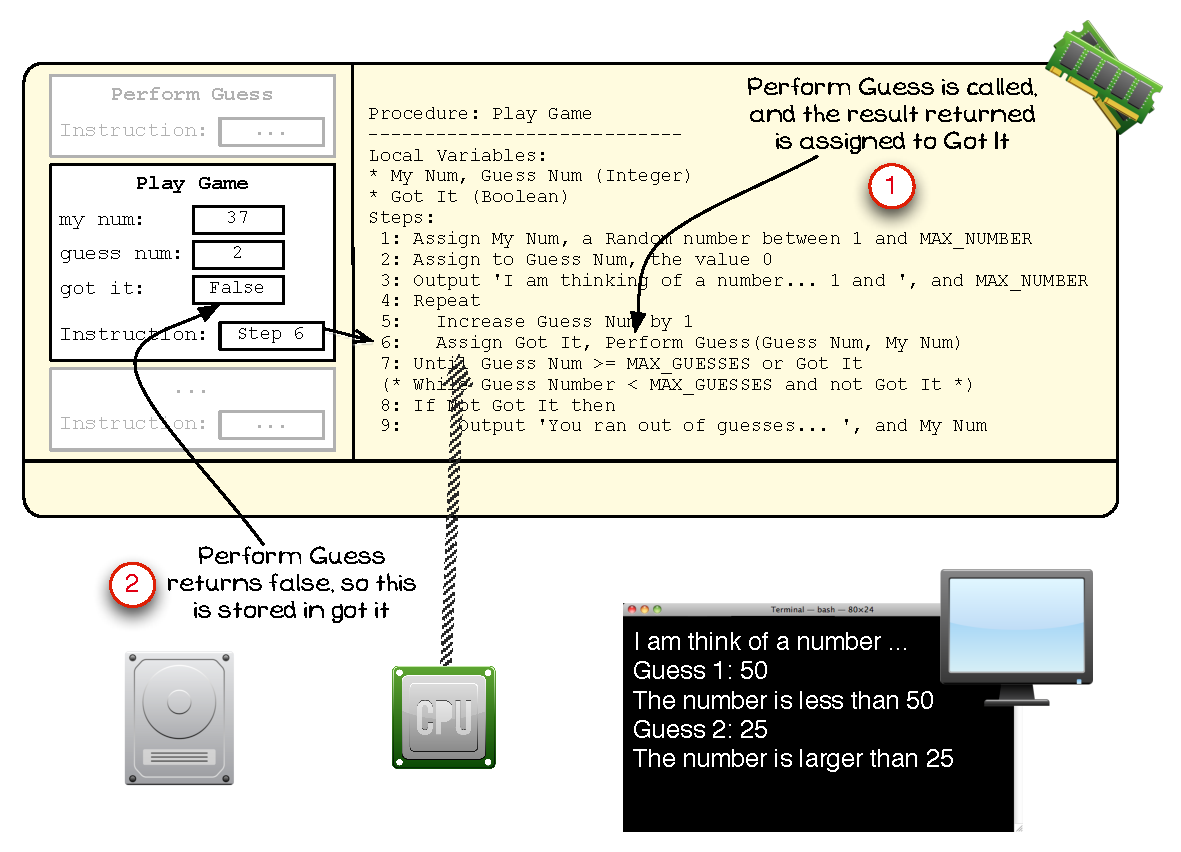
\includegraphics[width=\textwidth]{./topics/control-flow/images/PlayGame6} 
   \caption{\texttt{Perform Guess} is called again, it is passed 2 for its \texttt{guess num} and \texttt{37} for its \texttt{target} parameter}
   \label{fig:play-game-6}
\end{figure}

\mynote{
\begin{itemize}
  \item In \fref{fig:play-game-6} the indicated areas show the following:
  \begin{enumerate}
    \item This calls \texttt{Perform Guess} passing 2 to its \texttt{guess num} parameter, and 37 to its \texttt{target} parameter.
    \item \texttt{Perform Guess} returns \texttt{false}, indicating that the user did not guess the number.
  \end{enumerate}
  \medskip
  \item The following sections outline what occurred in this call to \texttt{Perform Guess}:
  \begin{enumerate}
    \item \nameref{ssub:perform_guess_is_called_for_guess_2}
    \item \nameref{ssub:if_takes_the_else_branch_for_guess_2}
    \item \nameref{ssub:the_inner_if_s_true_branch_is_taken_in_guess_2}
    \item \nameref{ssub:control_jumps_to_step_11_for_guess_2}
  \end{enumerate}
\end{itemize}
}

% subsubsection perform_guess_is_called_to_perform_guess_2 (end)

\clearpage
\subsubsection{Loop condition is checked at the end of guess 2, with the loop being repeated} % (fold)
\label{ssub:loop_condition_is_checked_at_the_end_of_guess_2}

The loop condition is checked again, and it indicates that the body needs to be repeated again.

\begin{figure}[htbp]
   \centering
   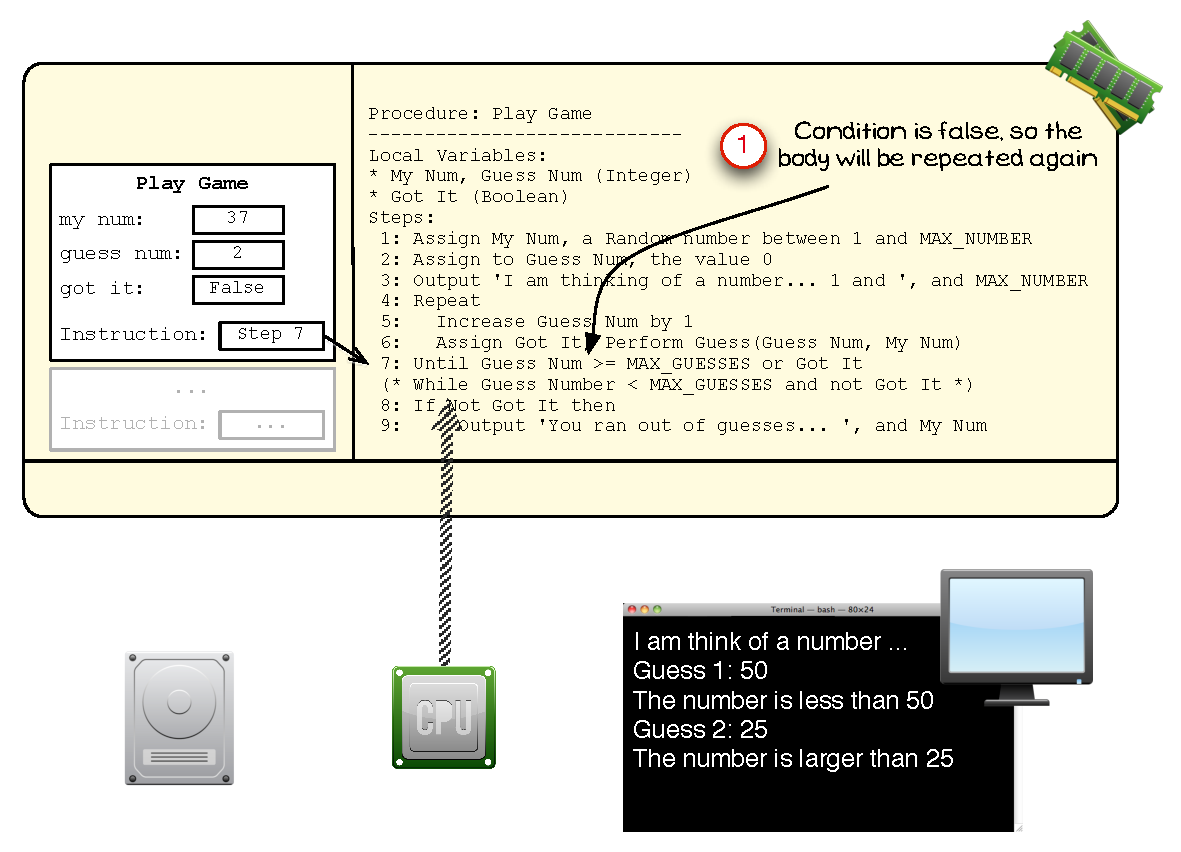
\includegraphics[width=\textwidth]{./topics/control-flow/images/PlayGame7} 
   \caption{}
   \label{fig:play-game-7}
\end{figure}

\mynote{
\begin{itemize}
  \item In \fref{fig:play-game-7} the indicated areas show the following:
  \begin{enumerate}
    \item The condition indicates that the loop's body needs to be repeated, allowing the user to enter guess 3.
  \end{enumerate}
  \medskip
  \item The same logic can be applied as shown in \nameref{ssub:loop_condition_is_checked_at_the_end_of_guess_1}.
  \item With \texttt{\textbf{repeat...until}} you can evaluate the expression by:
  \begin{enumerate}
    \item \csnipet{Guess Num >= MAX\_GUESSES} is \csnipet{2 >= 7}, this is \textbf{false}
    \item \texttt{Got it}, this is a variable, its value is \textbf{false}
    \item Or the above together, \passnipet{false or false}, this is \textbf{false}, repeating the loop.
  \end{enumerate}
  \item With \texttt{\textbf{do...while}} you can evaluate the expression by:
  \begin{enumerate}
    \item \csnipet{Guess Num < MAX\_GUESSES} is \csnipet{2 < 7}, this is \textbf{true}
    \item \texttt{Got it}, this is a variable, its value is \emph{false}, so \texttt{!Got it}, is \texttt{not false}, is \textbf{true}
    \item And together these results, \passnipet{true and true} is \textbf{true}, repeating the loop.
  \end{enumerate}
  
\end{itemize}
}

% subsubsection loop_condition_is_checked_at_the_end_of_guess_2 (end)

\clearpage
\subsubsection{\texttt{Perform Guess} is called a third time, and returns true for guess 3} % (fold)
\label{ssub:perform_guess_is_called_to_perform_guess_3}

Just as with guess 2, the body of the loop is repeated. Step 5 increases the value in \texttt{guess num} to 3 then control continues to step 6. This step calls \texttt{Perform Guess}, to allow the user to perform the third guess. This time around it is passed 3 for the \texttt{guess num}, and 37 for the \texttt{target}. When \texttt{Perform Guess} ends the result is now true, which is stored in \texttt{got it}.

\begin{figure}[htbp]
   \centering
   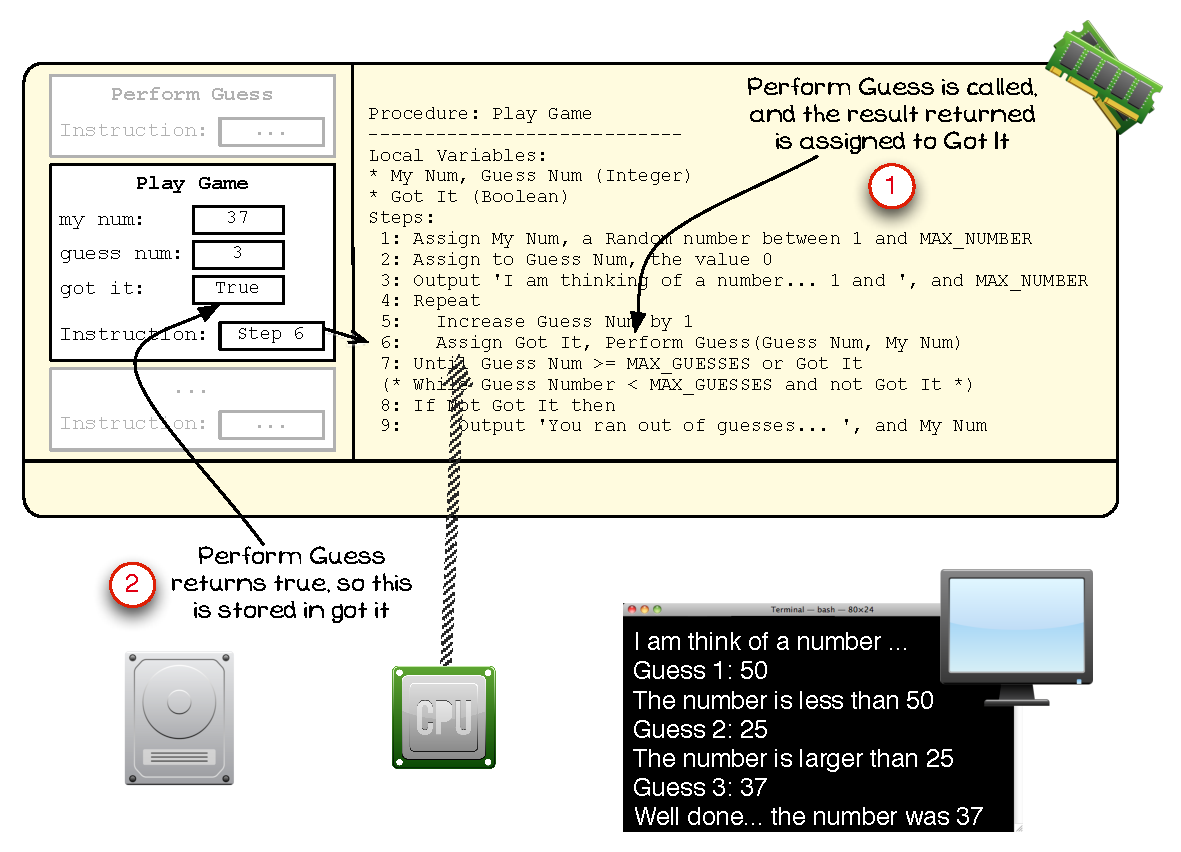
\includegraphics[width=\textwidth]{./topics/control-flow/images/PlayGame8} 
   \caption{\texttt{Perform Guess} is called for the third time, this time the user guesses the number}
   \label{fig:play-game-8}
\end{figure}

\mynote{
\begin{itemize}
  \item In \fref{fig:play-game-8} the indicated areas show the following:
  \begin{enumerate}
    \item This calls \texttt{Perform Guess} passing 3 to its \texttt{guess num} parameter, and 37 to its \texttt{target} parameter.
    \item \texttt{Perform Guess} returns \texttt{true}, indicating that the user has guessed the number. We now want the loop to end, as the number has been guessed.
  \end{enumerate}
  \medskip
  \item The following sections outline what occurred in this call to \texttt{Perform Guess}:
  \begin{enumerate}
    \item \nameref{ssub:perform_guess_is_called_again_for_guess_3}.
    \item \nameref{ssub:if_takes_the_else_branch_for_guess_3}.
    \item \nameref{ssub:the_inner_if_s_else_branch_is_taken_in_guess_3}.
    \item \nameref{ssub:control_jumps_to_step_11_for_guess_3}.
  \end{enumerate}
\end{itemize}
}

% subsubsection perform_guess_is_called_to_perform_guess_3 (end)

\clearpage
\subsubsection{Loop condition is checked at the end of guess 3, ending the loop} % (fold)
\label{ssub:loop_condition_is_checked_at_the_end_of_guess_3}

The loop condition is checked again, and this time it indicates that the loop should end.

\begin{figure}[htbp]
   \centering
   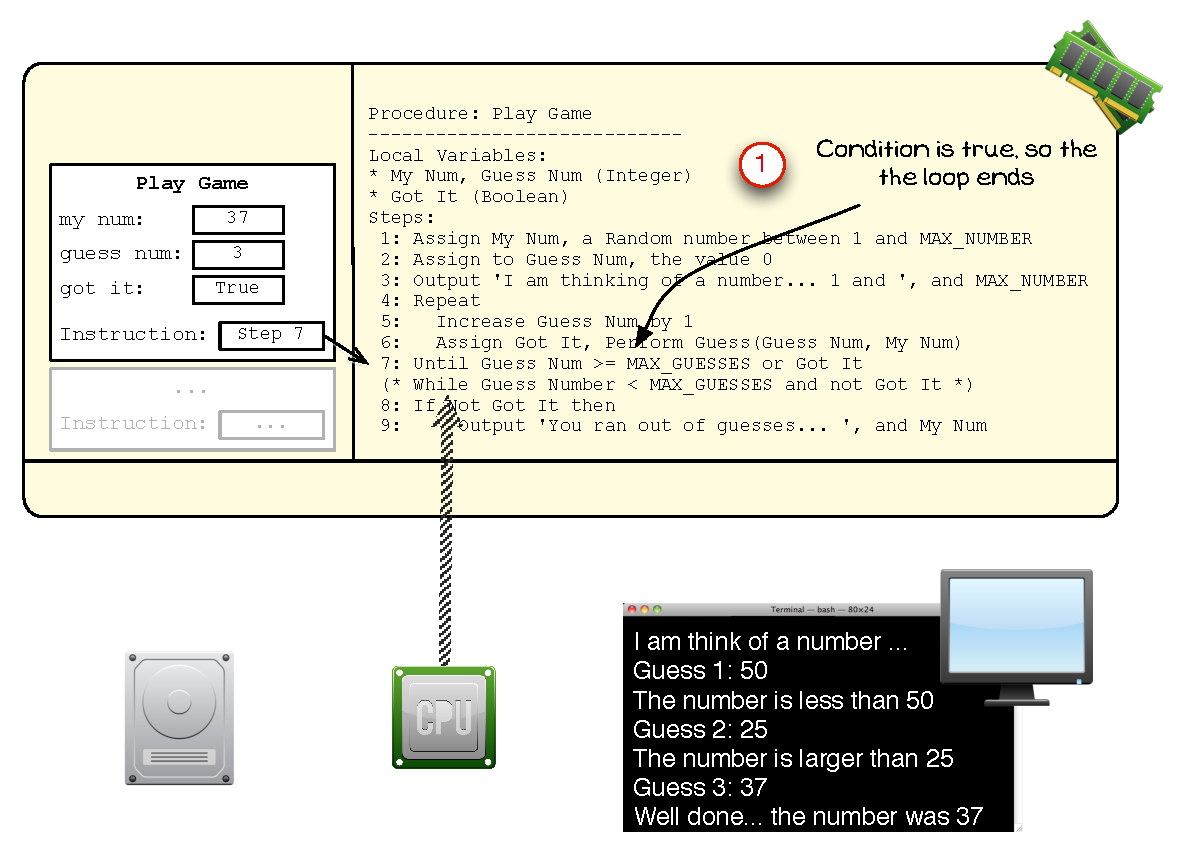
\includegraphics[width=\textwidth]{./topics/control-flow/images/PlayGame9} 
   \caption{Condition is checked, this time it indicates that the loop should end}
   \label{fig:play-game-9}
\end{figure}

\mynote{
\begin{itemize}
  \item In \fref{fig:play-game-9} the indicated areas show the following:
  \begin{enumerate}
    \item The condition indicates that the loop should end.
  \end{enumerate}
  \medskip
  \item With \texttt{\textbf{repeat...until}} you can evaluate the expression by:
  \begin{enumerate}
    \item \csnipet{Guess Num >= MAX\_GUESSES} is \csnipet{3 >= 7}, this is \textbf{false}
    \item \texttt{Got it}, this is a variable, its value is \textbf{true}
    \item Or the above together, \passnipet{false or true}, is \textbf{true}, ending the loop.
  \end{enumerate}
  \item With \texttt{\textbf{do...while}} you can evaluate the expression by:
  \begin{enumerate}
    \item \csnipet{Guess Num < MAX\_GUESSES} is \csnipet{3 < 7}, this is \textbf{true}
    \item \texttt{Got it}, this is a variable, its value is \emph{true}, so \texttt{!Got it}, is \texttt{not true}, is \textbf{false}
    \item And together these results, \passnipet{true and false} is \textbf{false}, ending the loop.
  \end{enumerate}
  \item Notice how the \texttt{got it} boolean is used to stop the loop when the user gets the answer. This is the purpose of this variable.
\end{itemize}
}

% subsubsection loop_condition_is_checked_at_the_end_of_guess_3 (end)

\clearpage
\subsubsection{Branch is checked after the loop} % (fold)
\label{ssub:branch_is_checked_after_the_loop}

The branch after the loop's body outputs the number if the user did not guess it.

\begin{figure}[htbp]
   \centering
   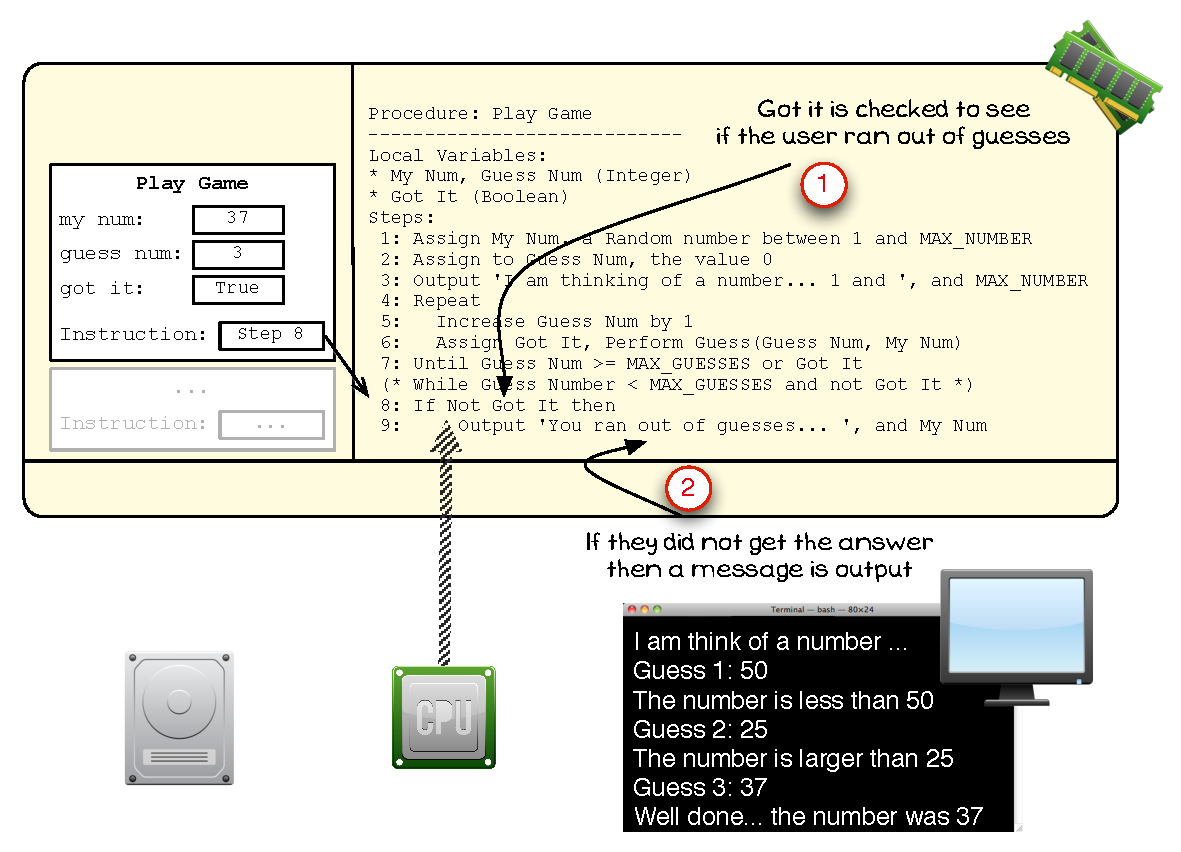
\includegraphics[width=\textwidth]{./topics/control-flow/images/PlayGame10} 
   \caption{Branch after the loop outputs the answer if the users did not guess the number}
   \label{fig:play-game-10}
\end{figure}

\mynote{
\begin{itemize}
  \item In \fref{fig:play-game-10} the indicated areas show the following:
  \begin{enumerate}
    \item The \nameref{sub:if_statement} checks if the user guessed the number (\texttt{got it}).
    \item If they did not guess the number then the number is output.
  \end{enumerate}
  \medskip
  \item In this case the condition is false, so the \emph{true} branch is skipped. This ends the if statement, and the procedure allowing control to return to the calling code.
  \item This needed to use \texttt{got it}, as the user may guess the number on the last guess.
\end{itemize}
}

% subsubsection branch_is_checked_after_the_loop (end)
% subsection understanding_looping_in_play_game (end)

\clearpage
\subsection{Understanding looping in Print Line} % (fold)
\label{sub:understanding_looping_in_print_line}

\fref{fig:print-line-understanding} shows the flowchart for the \texttt{Print Line} procedure that was developed in \sref{sub:designing_control_flow_for_print_line} on \nameref{sub:designing_control_flow_for_print_line}. The following sections outline how these actions are executed within the computer.

\begin{figure}[htbp]
   \centering
   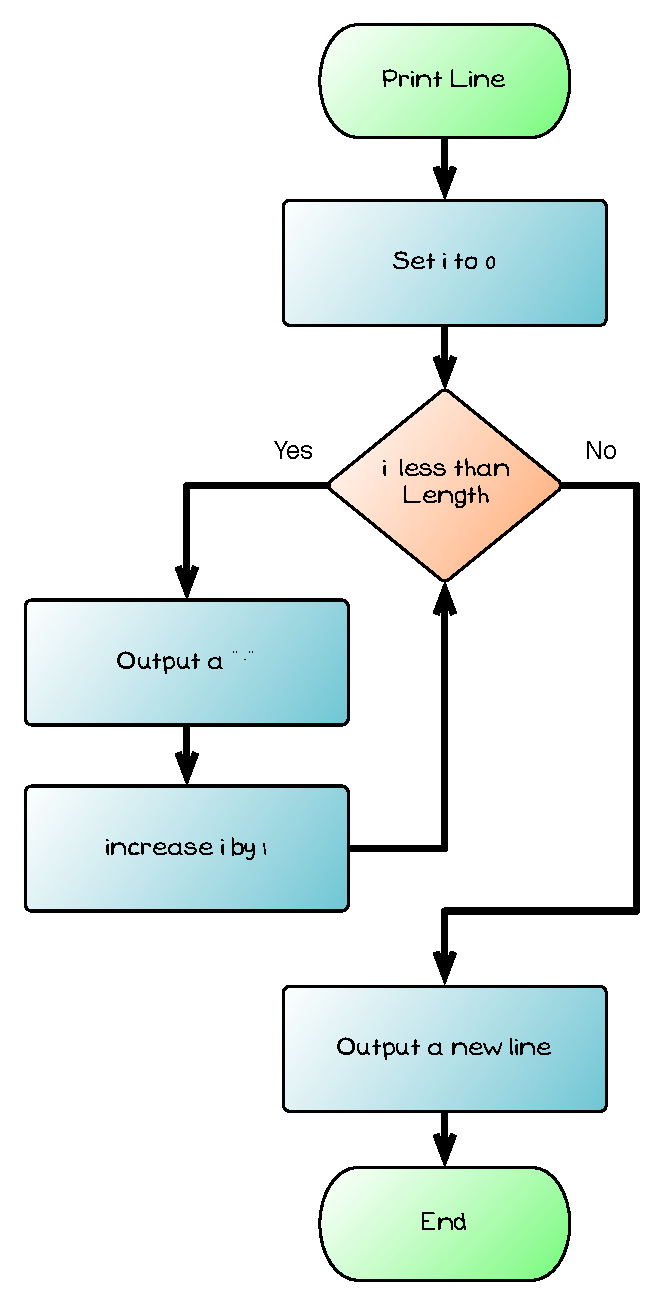
\includegraphics[width=0.4\textwidth]{./topics/control-flow/diagrams/PrintLine} 
   \caption{Logic for the \texttt{Print Line} Procedure from \fref{fig:print-line}}
   \label{fig:print-line-understanding}
\end{figure}

The illustrations will show a single execution of the \texttt{Print Line} procedure, with 3 being passed to its \texttt{length} parameter. This call will output a three line of dash characters, demonstrating how the \nameref{sub:pre_test_loop} differs from the \nameref{sub:post_test_loop}.

\clearpage
\subsubsection{Print Line is called to print a line of three characters} % (fold)
\label{ssub:print_line_is_called_to_print_a_line_of_three_characters}

The illustration starts with the call to \texttt{Print Line}. It is called to print a line of three dash (-) characters to the Terminal.

\begin{figure}[htbp]
   \centering
   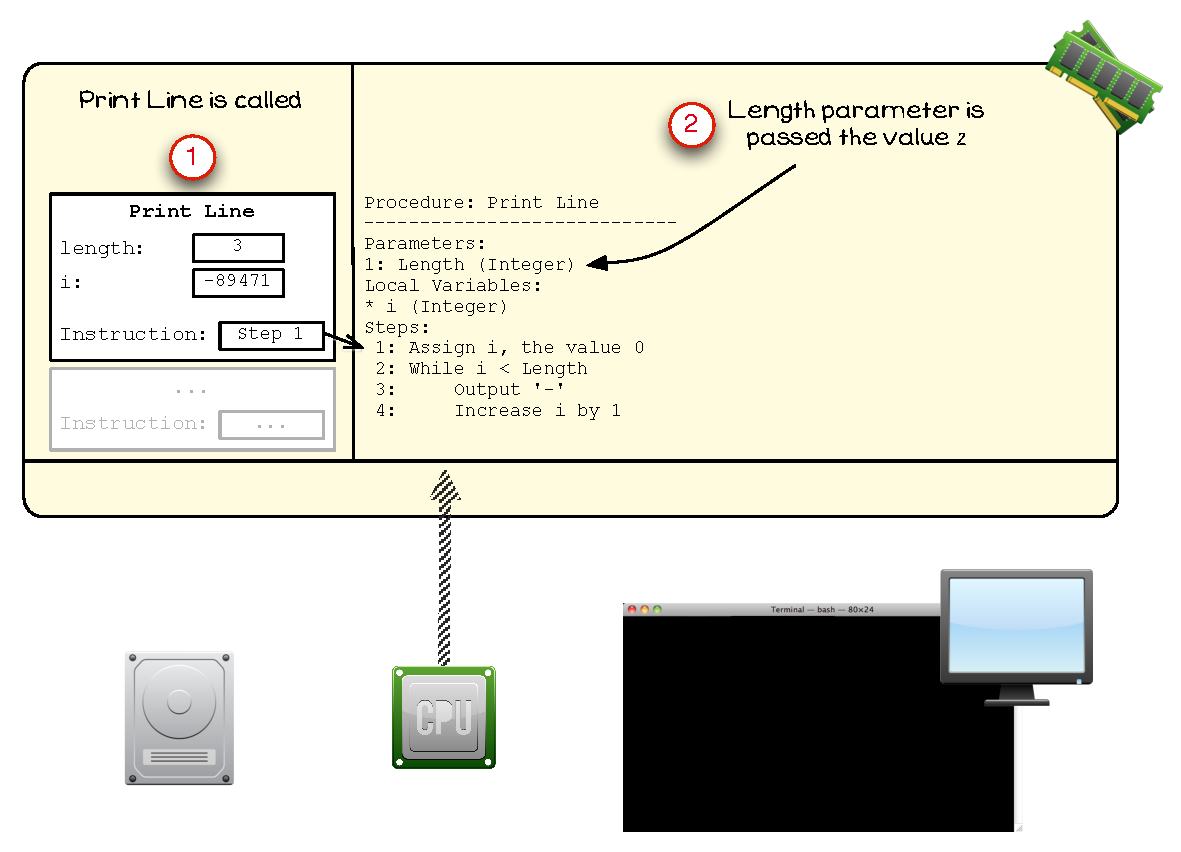
\includegraphics[width=\textwidth]{./topics/control-flow/images/PrintLine1} 
   \caption{\texttt{Print Line} starts, and is passed the value 3}
   \label{fig:print-line-1}
\end{figure}

\mynote{
\begin{itemize}
  \item In \fref{fig:print-line-1} the indicated areas show the following:
  \begin{enumerate}
    \item At some stage in the program \texttt{Print Line} is called, and its loaded onto the stack.
    \item The \texttt{length} parameter is passed the number of dash characters to be printed in the line. In this case that is 3.
  \end{enumerate}
  \medskip
  \item The \texttt{i} local variable is uninitialised, and has the value that was last at that location in memory.
\end{itemize}
}
% subsubsection print_line_is_called_to_print_a_line_of_three_characters (end)

\clearpage
\subsubsection{Execution proceeds to the while loop} % (fold)
\label{ssub:execution_proceeds_to_the_while_loop}

The first instructions are executed as normal, initialising the value of the \texttt{i} variable. At the \texttt{while} loop the computer checks the condition and determines that the loop should execute. This means that the next instruction will be taken from Step 3 of the code.

\begin{figure}[htbp]
   \centering
   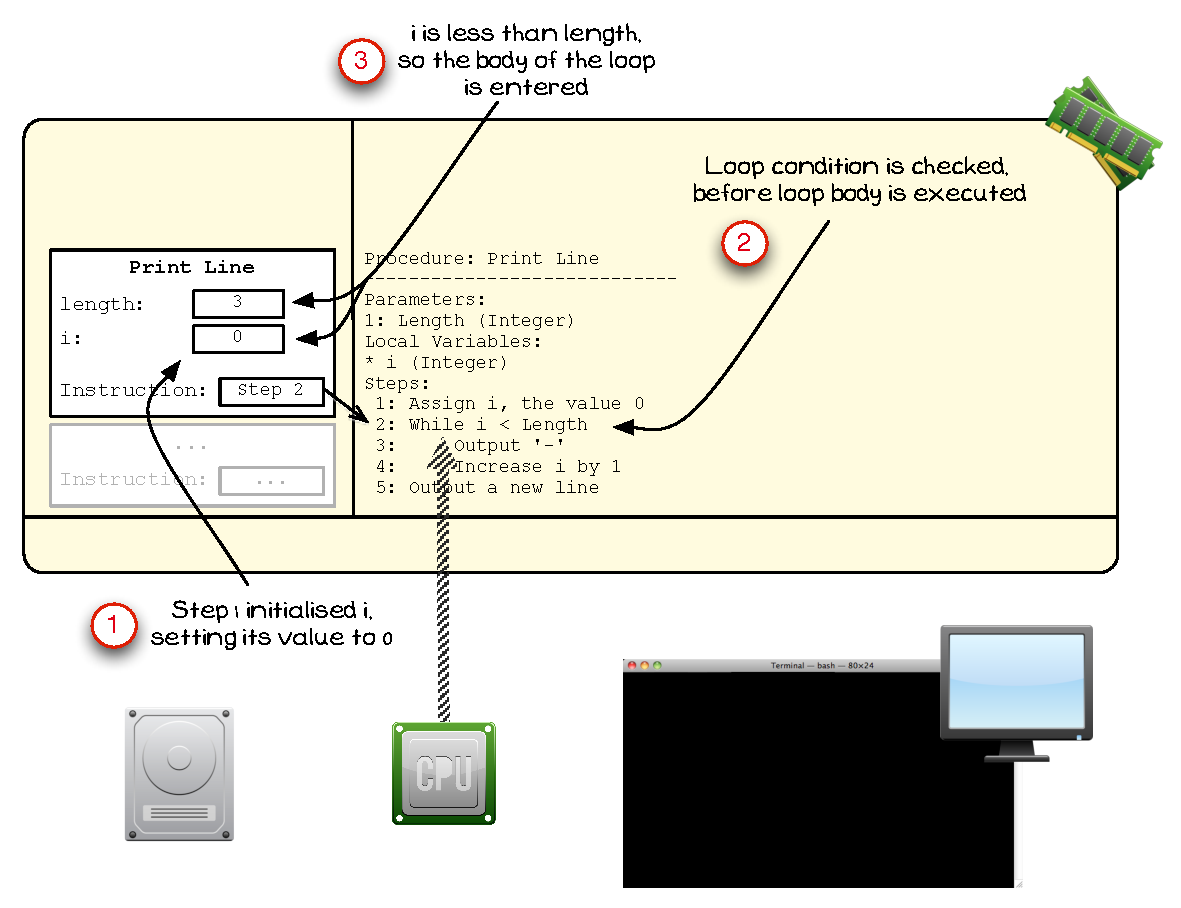
\includegraphics[width=\textwidth]{./topics/control-flow/images/PrintLine2} 
   \caption{\texttt{i} is initialised, and the loop checks its condition}
   \label{fig:print-line-2}
\end{figure}

\mynote{
\begin{itemize}
  \item In \fref{fig:print-line-2} the indicated areas show the following:
  \begin{enumerate}
    \item Step 1 assigns the value 0 to \texttt{i}.
    \item Step 2 checks the condition to determine which path to take. 
    \item As \texttt{i} \textbf{is less than} \texttt{length} control will flow to Step 3.
  \end{enumerate}
  \medskip
  \item The \texttt{while} loop only checks the condition at the start of the loop. It is at this point that it decides \emph{if} the code should enter the loop, or if it should end the loop by skipping the loop's body.
  \item In this case the condition indicate the loop should enter, so control enters the body of the loop.
\end{itemize}
}

% subsubsection execution_proceeds_to_the_while_loop (end)

\clearpage
\subsubsection{First dash is output to the Terminal} % (fold)
\label{ssub:first_dash_is_output_to_the_terminal}

The body of the loop is entered, and the first instruction (Step 3) outputs a dash to the Terminal.

\begin{figure}[htbp]
   \centering
   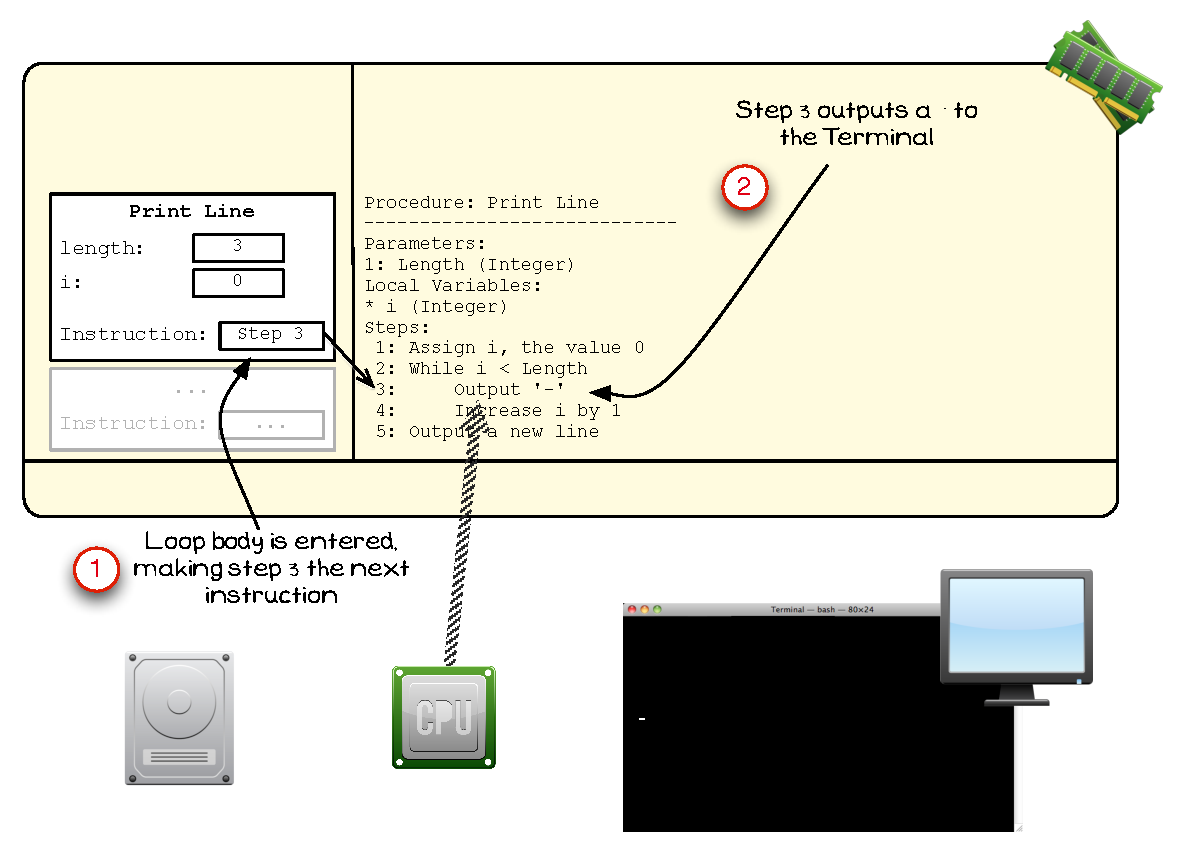
\includegraphics[width=\textwidth]{./topics/control-flow/images/PrintLine3} 
   \caption{The first dash is output to the Terminal}
   \label{fig:print-line-3}
\end{figure}

\mynote{
\begin{itemize}
  \item In \fref{fig:print-line-3} the indicated areas show the following:
  \begin{enumerate}
    \item The loop body starts at Step 3.
    \item This step outputs a dash to the Terminal.
  \end{enumerate}
  \medskip
  \item You could use this kind of loop to perform any action a number of times. The body of the loop is then performed once each time the loop executes.
\end{itemize}
}

% subsubsection first_dash_is_output_to_the_terminal (end)

\clearpage
\subsubsection{\texttt{i} is incremented, counting the number of times the loop has run} % (fold)
\label{ssub:i_is_incremented_to_count_the_loops}

After outputting the dash, the next instruction (Step 4) increments the value of \texttt{i}. In this code \texttt{i} is counting the number of times the loop has been performed. This is the end of the first loop, so now \texttt{i} has the value 1.

\begin{figure}[htbp]
   \centering
   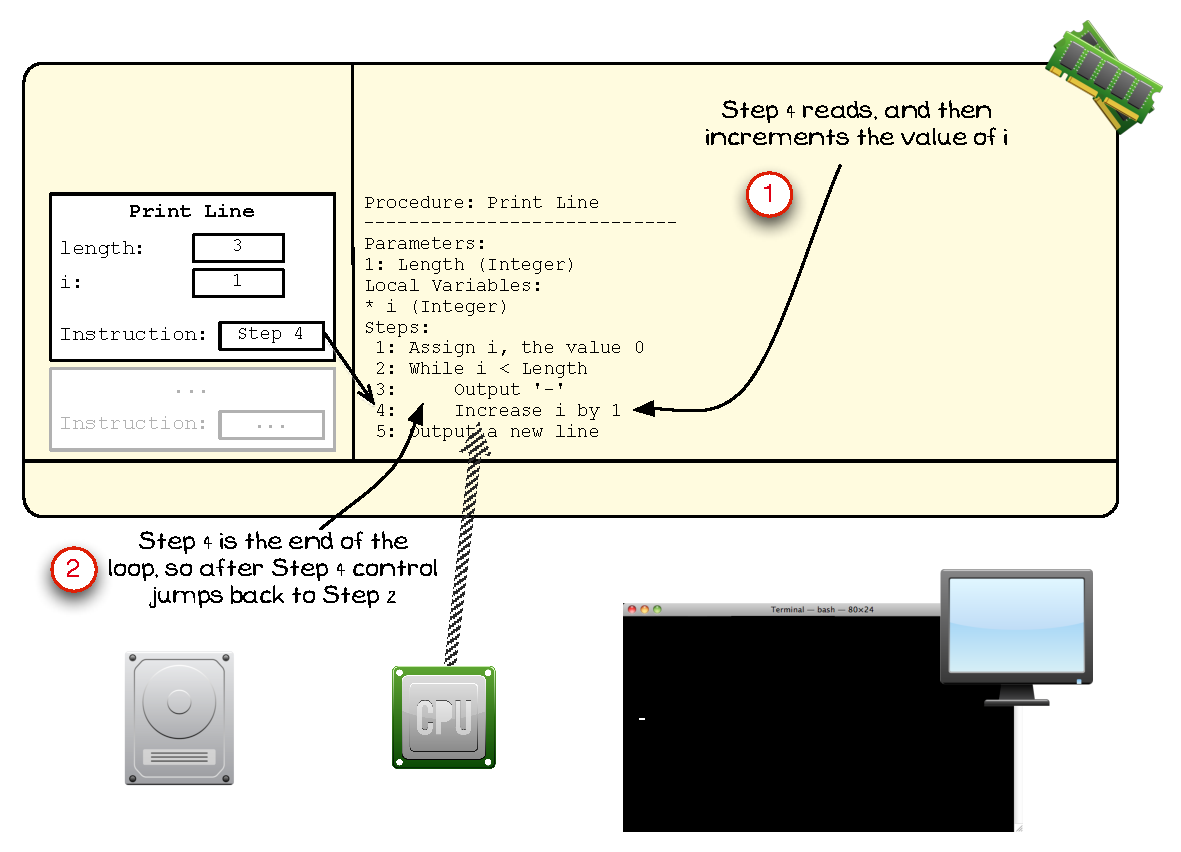
\includegraphics[width=\textwidth]{./topics/control-flow/images/PrintLine4} 
   \caption{\texttt{i} is keeping track of the number of times the loop has been performed}
   \label{fig:print-line-4}
\end{figure}

\mynote{
\begin{itemize}
  \item In \fref{fig:print-line-4} the indicated areas show the following:
  \begin{enumerate}
    \item Step 4 increments the value of \texttt{i}, allowing it to keep track of the number of times the loop has executed.
    \item Control has reached the end of the loop, but will now return back to the condition.
  \end{enumerate}
  \medskip
  \item The compiler adds jump code to the end of each \nameref{sub:pre_test_loop}. This returns control to the loop's condition, thereby making the loop.
  \item 
\end{itemize}
}

% subsubsection i_is_incremented_to_count_the_loops (end)
\clearpage

\subsubsection{Condition is checked again, and the body of the loop reentered} % (fold)
\label{ssub:condition_is_checked_again_and_the_body_of_the_loop_rentered}

The while loop checks the condition to determine if the body should be executed again, or if the loop should end. In this case \texttt{i} is still less than \texttt{length} so the body of the loop is executed again.

\begin{figure}[htbp]
   \centering
   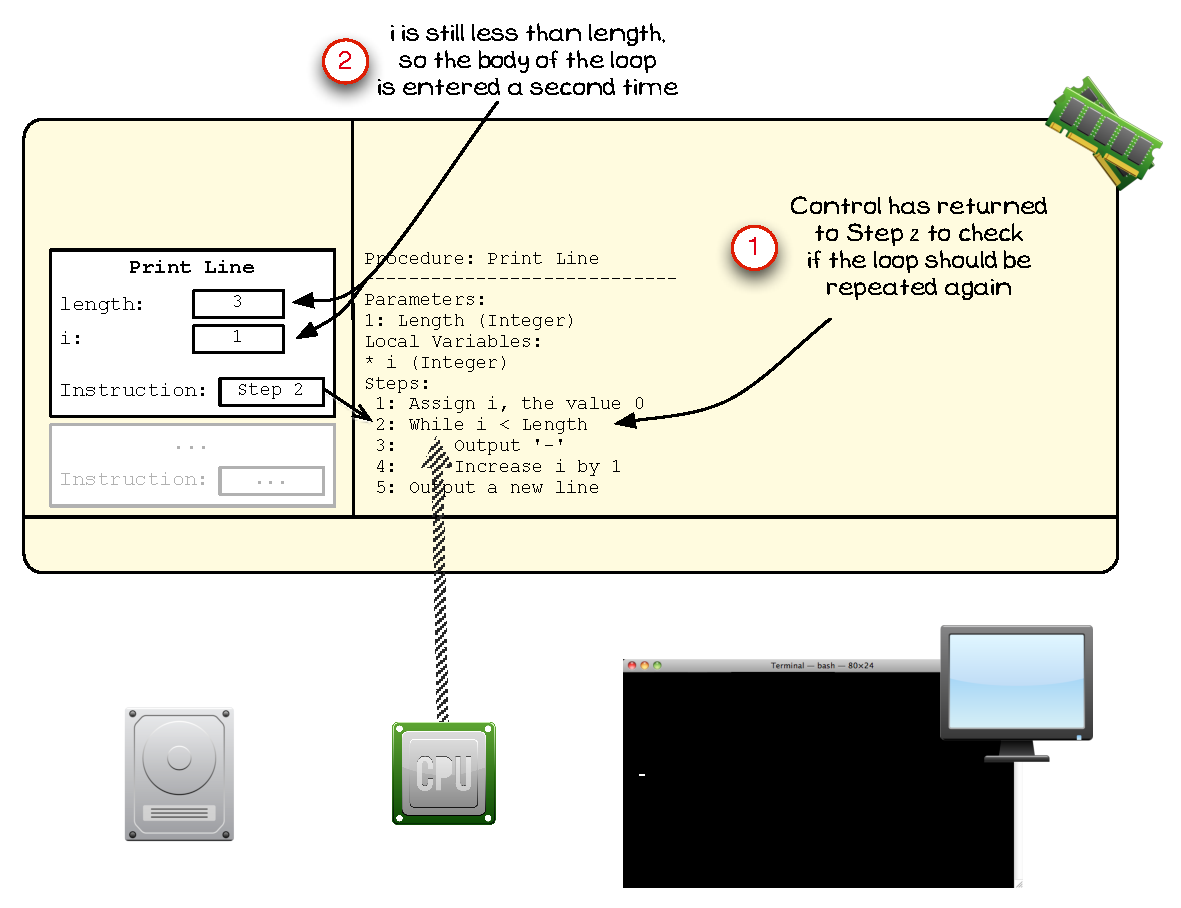
\includegraphics[width=\textwidth]{./topics/control-flow/images/PrintLine5} 
   \caption{Loop condition is checked to determine if the loop should run again}
   \label{fig:print-line-5}
\end{figure}

\mynote{
\begin{itemize}
  \item In \fref{fig:print-line-5} the indicated areas show the following:
  \begin{enumerate}
    \item The condition is checked again, to determine if the body is run or skipped.
    \item In this case the loop body is run again as \texttt{i} \textbf{is less than} \texttt{length}.
  \end{enumerate}
  \medskip
  \item The \nameref{sub:pre_test_loop} is controlled by the condition at the start of the loop.
\end{itemize}
}

% subsubsection condition_is_checked_again_and_the_body_of_the_loop_rentered (end)

\clearpage

\subsubsection{Loop 2 starts, outputting the second dash} % (fold)
\label{ssub:loop_2_starts_outputting_the_second_dash}

The loop body is run again with its first instruction (Step 3) outputting another dash to the Terminal.

\begin{figure}[htbp]
   \centering
   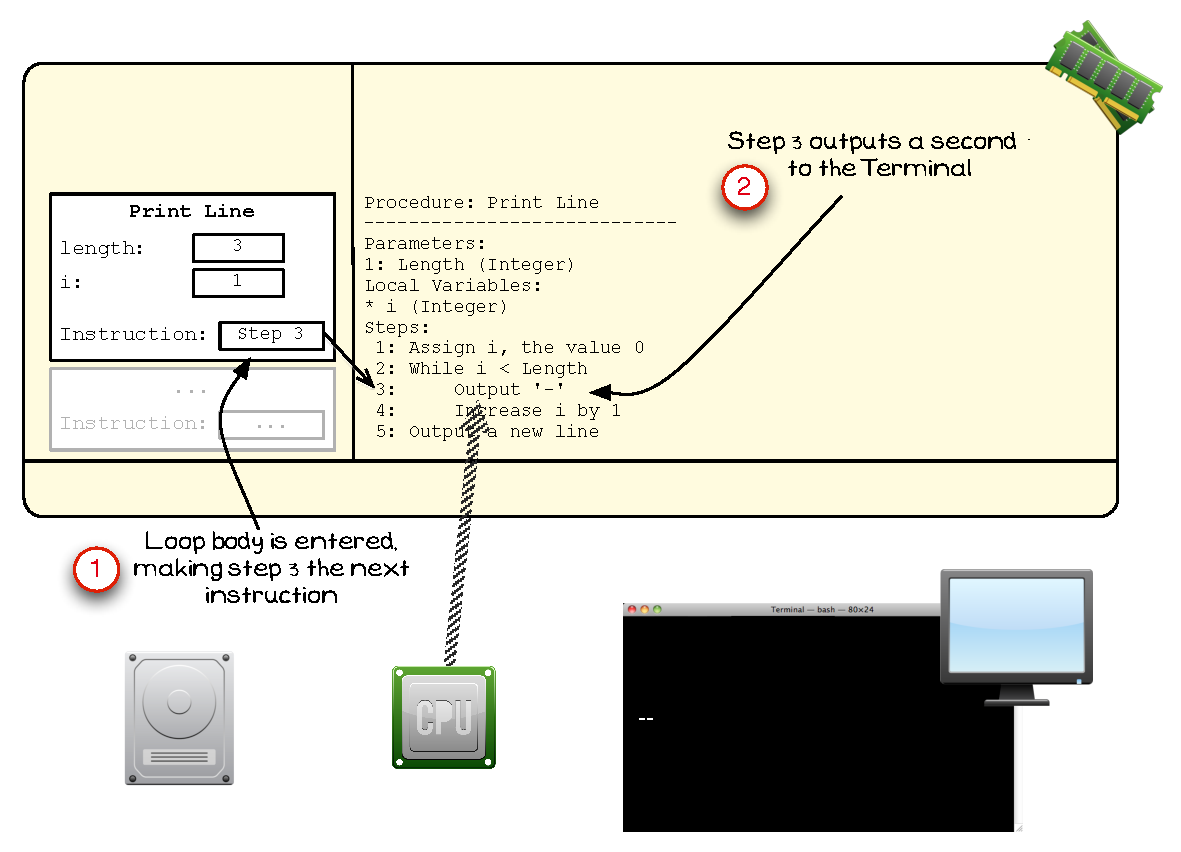
\includegraphics[width=\textwidth]{./topics/control-flow/images/PrintLine6} 
   \caption{The loop body is run again, and a second dash is output}
   \label{fig:print-line-6}
\end{figure}

\mynote{
\begin{itemize}
  \item In \fref{fig:print-line-6} the indicated areas show the following:
  \begin{enumerate}
    \item As before, the loop body starts at Step 3.
    \item This step outputs a second dash to the Terminal.
  \end{enumerate}
  \medskip
  \item All the instructions in this sequence will be executed each time the loop is repeated.
\end{itemize}
}

% subsubsection loop_2_starts_outputting_the_second_dash (end)
\clearpage

\subsubsection{\texttt{i} is incremented again, indicating that the loop has run twice} % (fold)
\label{ssub:i_is_incremented_again_indicating_that_the_loop_has_run_twice}

The last instruction in this sequence increments the value of \texttt{i}, indicating that the loop has run twice. Once again, control returns jumps back to the condition. It is the condition that will determine when the loop ends, the end of the loop just indicates that control will return back to the condition.

\begin{figure}[htbp]
   \centering
   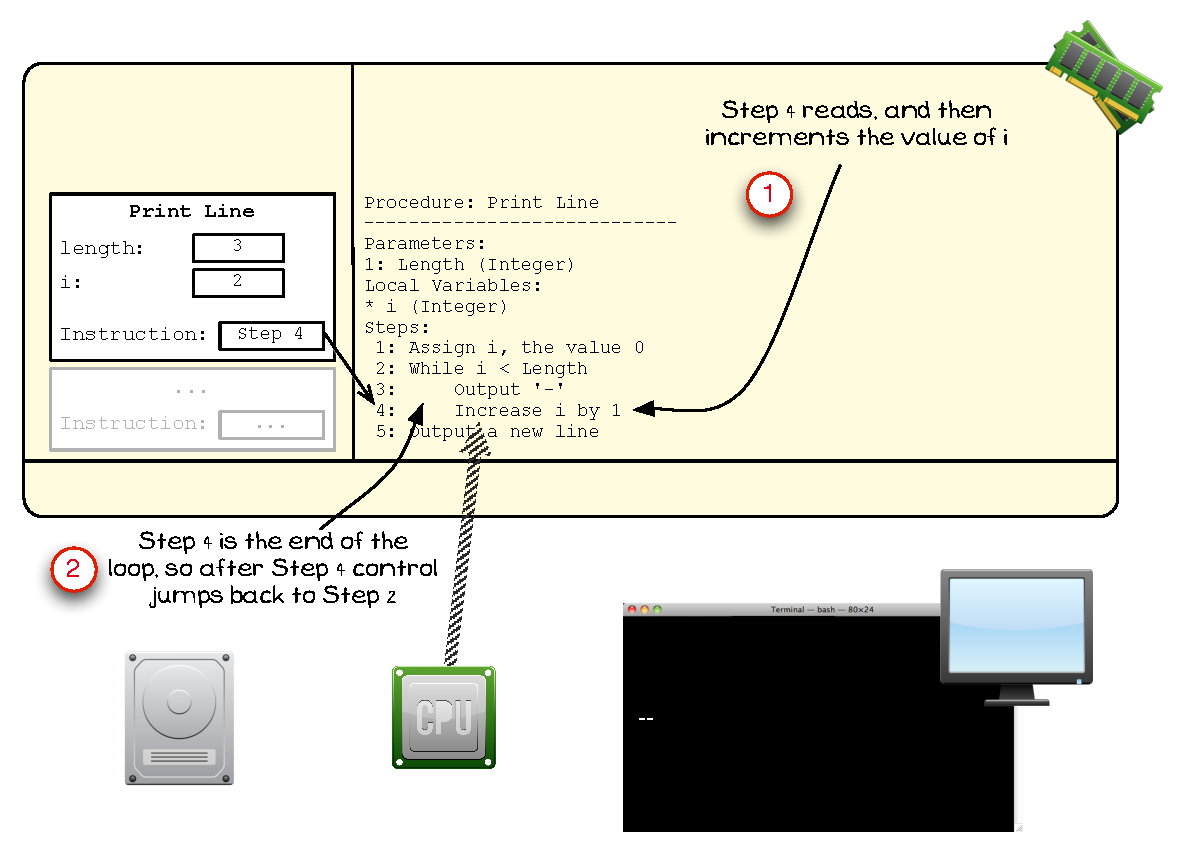
\includegraphics[width=\textwidth]{./topics/control-flow/images/PrintLine7} 
   \caption{\texttt{i} is incremented, and then control returns back to the loop's condition}
   \label{fig:print-line-7}
\end{figure}

\mynote{
\begin{itemize}
  \item In \fref{fig:print-line-7} the indicated areas show the following:
  \begin{enumerate}
    \item Step 4 increments the value of \texttt{i}. This is keeping track of the number of times through the loop, indicating that the loop has run twice.
    \item Control has reached the end of the loop and now jumps back to the condition.
  \end{enumerate}
  \medskip
  \item The \nameref{sub:post_test_loop} will always be performed in this way. The body of the loop runs, and then control jumps back to the condition.
\end{itemize}
}

% subsubsection i_is_incremented_again_indicating_that_the_loop_has_run_twice (end)
\clearpage

\subsubsection{Condition is checked again, and the loop runs a third time} % (fold)
\label{ssub:condition_is_checked_again_and_the_loop_runs_a_third_time}

When the condition is checked it determines if the loop body runs, or is skipped. In this case \texttt{i} is still less than \texttt{length} so the body is run a third time.

\begin{figure}[htbp]
   \centering
   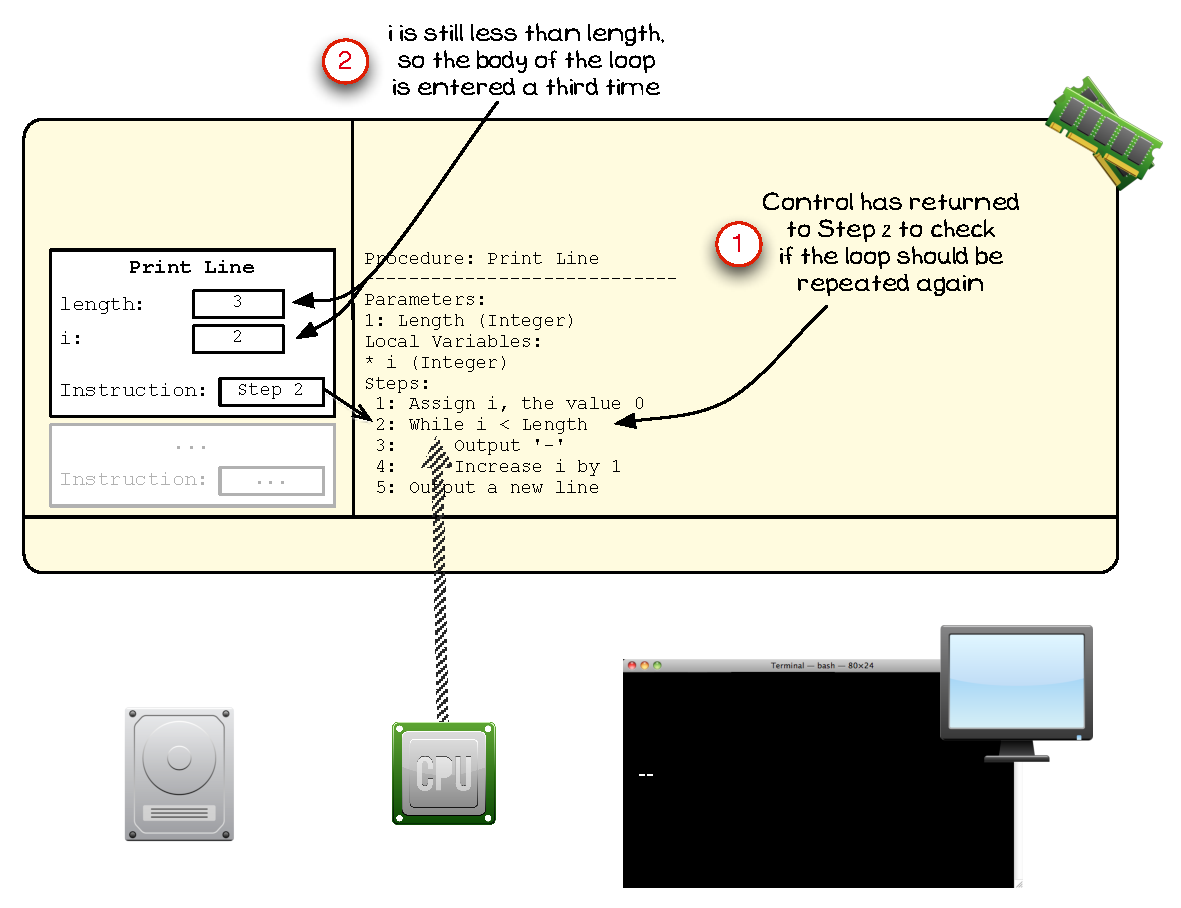
\includegraphics[width=\textwidth]{./topics/control-flow/images/PrintLine8} 
   \caption{While determines that the loop should run again}
   \label{fig:print-line-8}
\end{figure}

\mynote{
\begin{itemize}
  \item In \fref{fig:print-line-8} the indicated areas show the following:
  \begin{enumerate}
    \item The condition is checked again, to determine if the body is run or skipped.
    \item In this case the loop body is run again, as \texttt{i} \textbf{is less than} \texttt{length}.
  \end{enumerate}
  \medskip
  \item It is important to notice that this is only checked once each time the loop runs. It is checked when the condition is checked upon entry, and then again each time the loop jumps back to this step.
\end{itemize}
}

% subsubsection condition_is_checked_again_and_the_loop_runs_a_third_time (end)
\clearpage

\subsubsection{Another dash is output as the loop body runs a third time} % (fold)
\label{ssub:another_dash_is_output_as_the_loop_body_runs_a_third_time}

The loop body is entered a third time, and its sequence of instructions is executed. This outputs a third dash to the Terminal.

\begin{figure}[htbp]
   \centering
   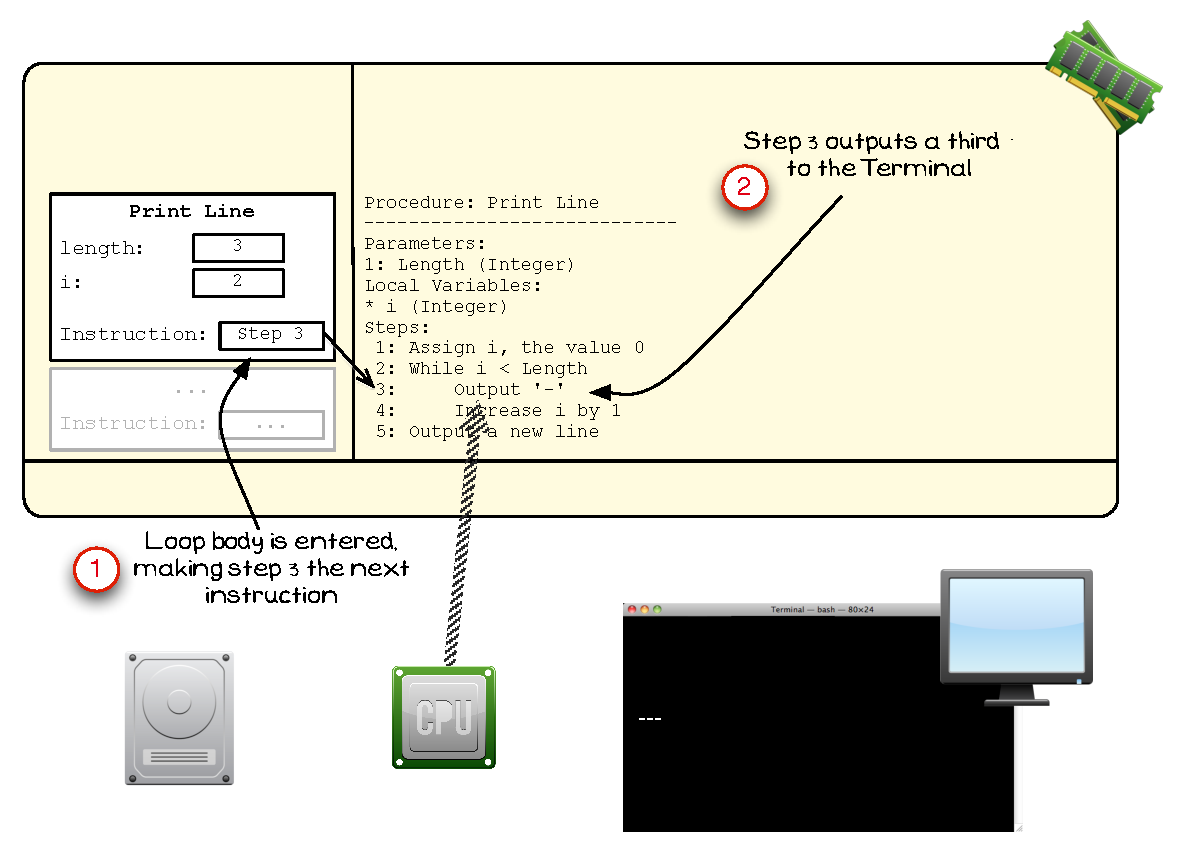
\includegraphics[width=\textwidth]{./topics/control-flow/images/PrintLine9} 
   \caption{The third dash is output to the Terminal}
   \label{fig:print-line-9}
\end{figure}

\mynote{
\begin{itemize}
  \item In \fref{fig:print-line-9} the indicated areas show the following:
  \begin{enumerate}
    \item As before, the loop body starts at Step 3.
    \item This step outputs a second dash to the Terminal.
  \end{enumerate}
  \medskip
  \item As before each instruction within the loop's body will be executed.
\end{itemize}
}

% subsubsection another_dash_is_output_as_the_loop_body_runs_a_third_time (end)
\clearpage

\subsubsection{\texttt{i} is incremented again, indicating the loop has been performed three times} % (fold)
\label{ssub:i_is_incremented_again_indicating_the_loop_has_been_performed_three_times}

When Step 4 is executed \texttt{i} is incremented again, and now has the value 3. As this is the end of the loop, control will jump back to condition.

\begin{figure}[htbp]
   \centering
   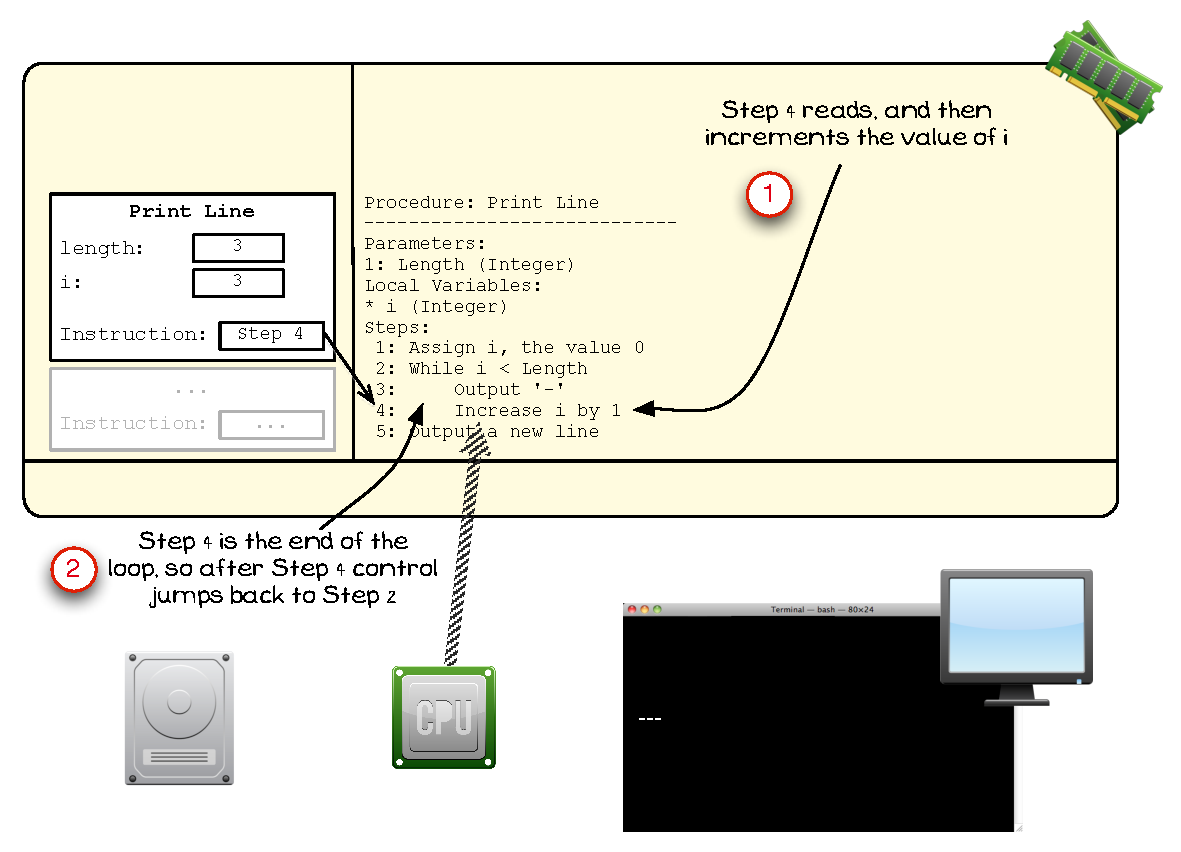
\includegraphics[width=\textwidth]{./topics/control-flow/images/PrintLine10} 
   \caption{\texttt{i} is incremented again, and then control jumps back to the condition}
   \label{fig:print-line-10}
\end{figure}

\mynote{
\begin{itemize}
  \item In \fref{fig:print-line-10} the indicated areas show the following:
  \begin{enumerate}
    \item Step 4 increments the value of \texttt{i}. This is keeping track of the number of times through the loop, indicating that the loop has run twice.
    \item Control has reached the end of the loop and now jumps back to the condition.
  \end{enumerate}
  \medskip
  \item The loop is controlled by the condition at the start, so it does not end at this point but it will end when the condition is next checked.
\end{itemize}
}

% subsubsection i_is_incremented_again_indicating_the_loop_has_been_performed_three_times (end)
\clearpage

\subsubsection{Condition is checked a fourth time, and the loop body is skipped} % (fold)
\label{ssub:condition_is_checked_a_fourth_time_and_the_loop_body_is_skipped}

The condition is checked again, and this time \texttt{i} \textbf{is not} less than \texttt{length} and so the loop body is not run again. Instead the computer jumps to the first instruction after the loop, Step 5. 

\begin{figure}[htbp]
   \centering
   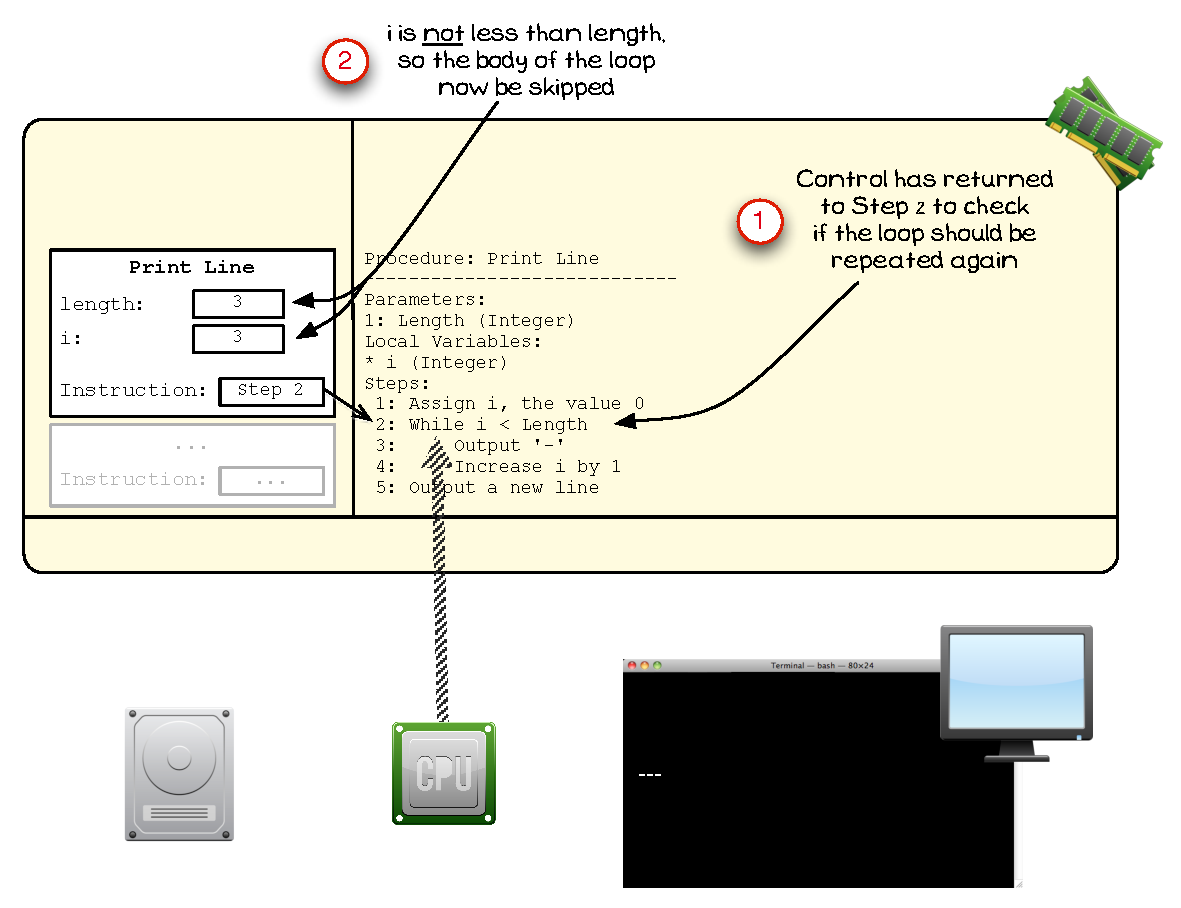
\includegraphics[width=\textwidth]{./topics/control-flow/images/PrintLine11} 
   \caption{The condition is now false, and so the computer jumps past the loop body to Step 5}
   \label{fig:print-line-11}
\end{figure}

\mynote{
\begin{itemize}
  \item In \fref{fig:print-line-11} the indicated areas show the following:
  \begin{enumerate}
    \item After the loop body completes, control \textbf{always} returns back to the start of the loop. It is this check that is controlling the loop, and it is only performed at this point.
    \item At this point \texttt{i} \textbf{is not less than} \texttt{length}, and therefore the body of the loop must be skipped.
  \end{enumerate}
  \medskip
  \item The next instruction will be Step 5, the first instruction past the end of the loop. This is the \textbf{single exit} point from the loop.
\end{itemize}
}

% subsubsection condition_is_checked_a_fourth_time_and_the_loop_body_is_skipped (end)
\clearpage

\subsubsection{Having completed the loop, the next instruction outputs a new line} % (fold)
\label{ssub:having_completed_the_loop_the_next_instruction_outputs_a_new_line}

Now that the loop has finished, control continues running the sequence from the Procedure.

\begin{figure}[htbp]
   \centering
   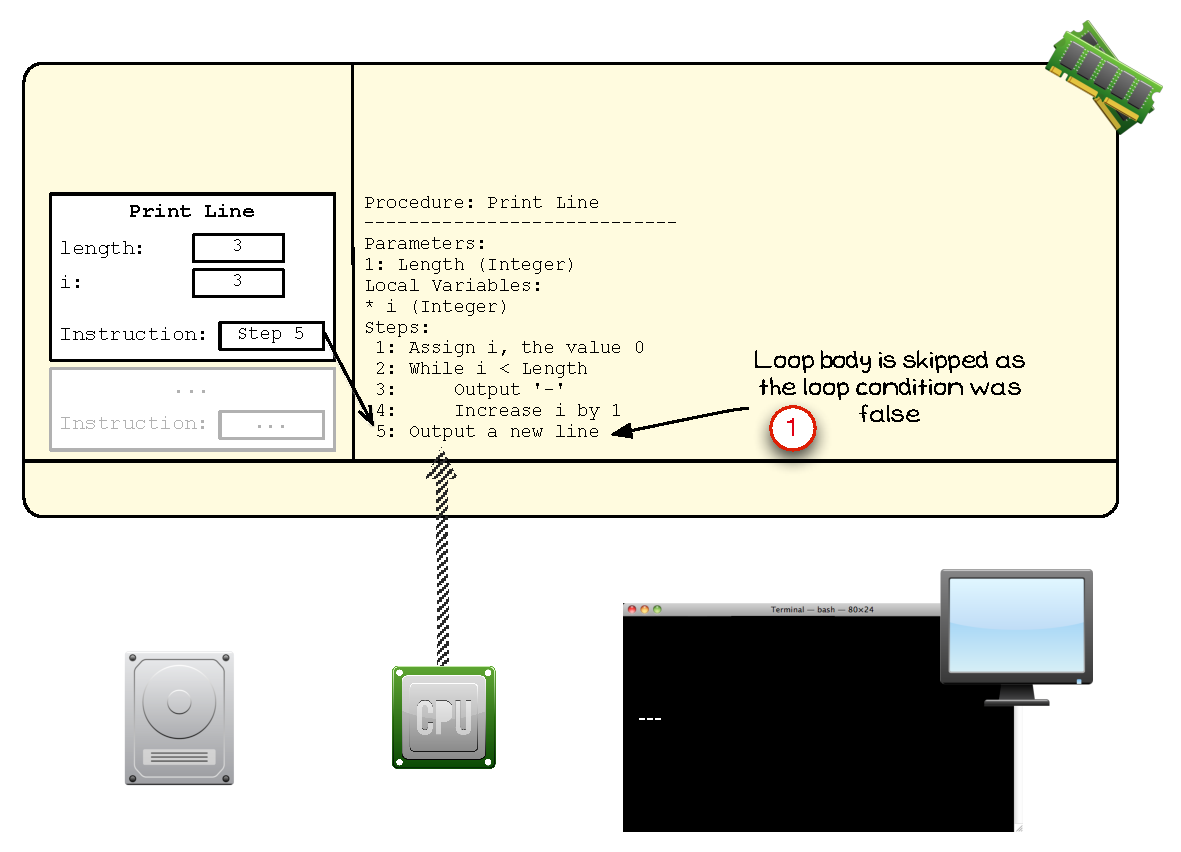
\includegraphics[width=\textwidth]{./topics/control-flow/images/PrintLine12} 
   \caption{Processing continues after the loop}
   \label{fig:print-line-12}
\end{figure}

\mynote{
\begin{itemize}
  \item In \fref{fig:print-line-12} the indicated areas show the following:
  \begin{enumerate}
    \item The condition indicates that the loop has ended, and so the next instruction is Step 5. This step outputs a new line, ending the line being printed to the Terminal.
  \end{enumerate}
  \medskip
  \item Notice how the condition controlled the behaviour of the loop. Each time it is checked it determines if the body is run again, or if it is skipped. 
  \item The condition is only checked once each loop: once at the start, and then once after each time through the loop body.
\end{itemize}
}

% subsubsection having_completed_the_loop_the_next_instruction_outputs_a_new_line (end)

% subsection understanding_looping_in_print_line (end)